% =====================================================================
% main.tex
% Responsabilidad única: ensamblar el documento completo a partir de los
% módulos (preámbulo, portada y las diez secciones de ejercicios). No
% contiene desarrollo matemático ni resultados propios — solo estructura.
%
% Para compilar:  latexmk -pdf main.tex
% =====================================================================
\documentclass[11pt]{article}

% =====================================================================
% preambulo.tex
% Responsabilidad única: cargar paquetes y definir configuración/estilos
% reutilizables (colores de enlaces, entornos, listas). No contiene
% contenido propio del taller — si algo del "look" del documento debe
% cambiar, este es el único archivo que hay que tocar.
% =====================================================================

\usepackage[utf8]{inputenc}
\usepackage[T1]{fontenc}
\usepackage[spanish,es-noshorthands,es-tabla]{babel}
\usepackage[a4paper,margin=2.5cm]{geometry}

% --- Matemáticas ------------------------------------------------------
\usepackage{amsmath}
\usepackage{amssymb}
\usepackage{amsthm}
\usepackage{mathtools}

% --- Tablas y figuras ---------------------------------------------------
\usepackage{graphicx}
\usepackage{booktabs}
\usepackage{array}
\usepackage{multirow}
\usepackage{caption}
\usepackage{float}
\usepackage{pgfplots}
\pgfplotsset{compat=1.18}

% --- Listas con formato a., b., c. ------------------------------------
\usepackage{enumitem}

% --- Diagramas vectoriales -----------------------------------------------
\usepackage{tikz}
\usetikzlibrary{arrows.meta, positioning, calc}
% Misma paleta usada en las figuras generadas con matplotlib (Ejercicios
% 6-10), para que los diagramas TikZ se vean como parte del mismo documento.
\definecolor{classblue}{HTML}{4C72B0}
\definecolor{classred}{HTML}{C44E52}
\definecolor{classgreen}{HTML}{55A868}

% --- Color y enlaces ----------------------------------------------------
\usepackage{xcolor}
\definecolor{urosariored}{RGB}{255,11,38} % rojo exacto muestreado del escudo
\usepackage{hyperref}
\hypersetup{
    colorlinks = true,
    linkcolor  = urosariored!75!black,
    citecolor  = urosariored!75!black,
    urlcolor   = urosariored!75!black,
    pdftitle   = {Taller 2 -- Modelos de aprendizaje supervisado},
    pdfauthor  = {Tania Fernanda Mora Cubillos, Over Haider Castrillon Valencia},
}

% --- Espaciado de tablas ------------------------------------------------
\renewcommand{\arraystretch}{1.25}

% --- Pie de página institucional -----------------------------------------
% Responsabilidad de este bloque: mostrar el escudo de la Universidad del
% Rosario, pequeño, en la esquina inferior derecha de cada página del
% cuerpo del documento (la portada define su propio pie por separado en
% portada.tex, ya que \begin{titlepage} usa página sin estilo).
\usepackage{fancyhdr}
\pagestyle{fancy}
\fancyhf{}
\renewcommand{\headrulewidth}{0pt}
\renewcommand{\footrulewidth}{0pt}
\fancyfoot[C]{\thepage}
\fancyfoot[R]{
\includegraphics[height=0.42cm]{figuras/logo_urosario_icono.png}}

% --- Encabezados de subsección sin numerar, para incisos a-e -----------
\setlist[enumerate,1]{label=\alph*., leftmargin=1.6em}

% --- Cifras generadas por el notebook -------------------------------------
% Responsabilidad de este bloque: cargar las macros con los resultados
% numéricos de los ejercicios 6-10 que escribe el notebook al ejecutarse
% (generado/resultados.tex), de modo que el texto cite \macro en lugar de
% copiar números a mano. Si el archivo aún no existe, se compila igual.
\InputIfFileExists{generado/resultados}{}{}


\begin{document}

% =====================================================================
% portada.tex
% Responsabilidad única: presentar los datos identificativos del taller
% (título, curso, estudiantes, profesor, fecha). No contiene desarrollo
% matemático ni resultados.
% =====================================================================

\begin{titlepage}
    \centering
    \vspace*{2cm}

    {\LARGE \textbf{Taller 2: Modelos de aprendizaje supervisado}}\\[0.4cm]
    {\normalsize\itshape Regresión lineal simple y múltiple, regresión logística y árboles de decisión}\\[0.6cm]
    {\large Aprendizaje Automático de Máquina I}\\[0.15cm]
    {\large Semestre 2026-2}\\[1.6cm]

    \rule{0.8\textwidth}{0.4pt}\\[0.9cm]

    \begin{tabular}{rl}
        \textbf{Estudiantes:}   & Tania Fernanda Mora Cubillos \\
                                & \small\texttt{taniaf.mora@urosario.edu.co} \\[0.35em]
                                & Over Haider Castrillón Valencia \\
                                & \small\texttt{over.castrillon@urosario.edu.co} \\[0.35em]
        \textbf{Programa:}      & Maestría en Matemáticas y Ciencias de la Computación \\[0.35em]
        \textbf{Profesor:}      & Daniel Felipe Rambaut Lemus \\[0.35em]
        \textbf{Modalidad:}     & Grupal \\[0.35em]
        \textbf{Fecha:}         & \today \\
    \end{tabular}

    \vfill
    
\includegraphics[width=2.6cm]{figuras/logo_urosario.png}
\end{titlepage}


\tableofcontents
\newpage

% ---------------------------------------------------------------------
% Parte I — Componente teórico-matemático
% ---------------------------------------------------------------------
\section{Componente teórico-matemático}
% =====================================================================
% ejercicio01.tex
% Responsabilidad única: derivar las ecuaciones normales de la recta de
% mínimos cuadrados, ajustar los datos didácticos, verificar propiedades
% de los residuos y estudiar el efecto de una observación influyente.
% Cifras verificadas con verificacion/teoria.py.
% =====================================================================
\subsection{Ejercicio 1: Regresión lineal simple, ajuste e influencia de una observación}

\paragraph{La situación.} Una empresa quiere saber cuánta energía consume
un equipo según las horas que pasa encendido. Para cada uno de $n=5$ días
anotamos las horas de funcionamiento $x_i$ y el consumo $y_i$ en kWh:

\begin{table}[H]
\centering
\begin{tabular}{c|ccccc}
\toprule
Día $i$ & 1 & 2 & 3 & 4 & 5 \\
\midrule
Horas $x_i$ & 1 & 2 & 3 & 4 & 5 \\
Consumo $y_i$ (kWh) & 2 & 4 & 5 & 4 & 5 \\
\bottomrule
\end{tabular}
\caption{Datos del Ejercicio 1.}
\label{tab:ej1-datos}
\end{table}

Queremos resumir la relación con una recta
$\hat y_i=\beta_0+\beta_1x_i$, donde $\beta_0$ (el \emph{intercepto}) es la
altura de la recta cuando $x=0$ y $\beta_1$ (la \emph{pendiente}) es cuánto
sube el consumo predicho por cada hora adicional. Ninguna recta pasa por
los cinco puntos, así que cada predicción tendrá un error
$y_i-\hat y_i$. El criterio de \emph{mínimos cuadrados} elige la recta que
hace más pequeña la suma de esos errores elevados al cuadrado,
\[
    S(\beta_0,\beta_1)=\sum_{i=1}^{n}\bigl(y_i-\beta_0-\beta_1x_i\bigr)^2 .
\]
Elevar al cuadrado cumple dos funciones: evita que los errores positivos y
negativos se cancelen entre sí y castiga mucho más un error grande que
varios pequeños (un error de $4$ cuenta $16$, mientras que dos errores de
$2$ cuentan $4+4=8$).

\begin{enumerate}

\item \textbf{Ecuaciones normales y estimadores.}
$S$ es una función de dos variables, $\beta_0$ y $\beta_1$, que tiene forma
de tazón. En el fondo del tazón la superficie es plana en todas las
direcciones, así que ahí las dos derivadas parciales valen cero. Para
derivar usamos la regla de la cadena: la derivada de $(u)^2$ es $2u$
multiplicado por la derivada de $u$.

\emph{Paso 1: derivada respecto a $\beta_0$.} Dentro del paréntesis,
$u_i=y_i-\beta_0-\beta_1x_i$, cuya derivada respecto a $\beta_0$ es $-1$,
luego
\[
    \frac{\partial S}{\partial \beta_0}
    = \sum_i 2\,(y_i-\beta_0-\beta_1x_i)\cdot(-1)
    = -2\sum_i (y_i-\beta_0-\beta_1x_i) .
\]

\emph{Paso 2: derivada respecto a $\beta_1$.} Ahora la derivada de $u_i$
respecto a $\beta_1$ es $-x_i$, luego
\[
    \frac{\partial S}{\partial \beta_1}
    = \sum_i 2\,(y_i-\beta_0-\beta_1x_i)\cdot(-x_i)
    = -2\sum_i x_i(y_i-\beta_0-\beta_1x_i) .
\]

\emph{Paso 3: igualar a cero y ordenar.} Al igualar ambas a cero podemos
dividir entre $-2$ y repartir la suma término a término (recordando que
$\sum_i\beta_0=n\beta_0$, pues $\beta_0$ se suma $n$ veces):
\begin{align*}
    \sum_i y_i - n\beta_0 - \beta_1\sum_i x_i = 0
    &\quad\Longrightarrow\quad
    n\beta_0 + \beta_1\sum_i x_i = \sum_i y_i, \\
    \sum_i x_iy_i - \beta_0\sum_i x_i - \beta_1\sum_i x_i^2 = 0
    &\quad\Longrightarrow\quad
    \beta_0\sum_i x_i + \beta_1\sum_i x_i^2 = \sum_i x_iy_i .
\end{align*}
Estas dos igualdades son las \emph{ecuaciones normales}: un sistema de dos
ecuaciones con dos incógnitas.

\emph{Paso 4: despejar $\beta_0$.} Dividimos la primera ecuación entre $n$
y usamos que $\frac1n\sum_i x_i=\bar x$ y $\frac1n\sum_i y_i=\bar y$:
\[
    \beta_0 + \beta_1\bar x = \bar y
    \quad\Longrightarrow\quad
    \beta_0=\bar y-\beta_1\bar x .
\]
Esto dice algo útil por sí solo: la recta ajustada siempre pasa por el
punto de promedios $(\bar x,\bar y)$, porque al reemplazar $x=\bar x$
queda $\hat y=\bar y-\beta_1\bar x+\beta_1\bar x=\bar y$.

\emph{Paso 5: despejar $\beta_1$.} Sustituimos $\beta_0=\bar y-\beta_1\bar x$
en la segunda ecuación y usamos $\sum_i x_i=n\bar x$:
\begin{align*}
    (\bar y-\beta_1\bar x)\,n\bar x + \beta_1\sum_i x_i^2 &= \sum_i x_iy_i \\
    n\bar x\bar y - \beta_1 n\bar x^2 + \beta_1\sum_i x_i^2 &= \sum_i x_iy_i \\
    \beta_1\Bigl(\sum_i x_i^2 - n\bar x^2\Bigr) &= \sum_i x_iy_i - n\bar x\bar y .
\end{align*}

\emph{Paso 6: escribirlo con desviaciones.} Las dos expresiones entre
paréntesis se pueden escribir de forma más intuitiva. Expandiendo el
cuadrado y usando de nuevo $\sum_i x_i=n\bar x$,
\[
    \sum_i (x_i-\bar x)^2
    = \sum_i x_i^2 - 2\bar x\sum_i x_i + n\bar x^2
    = \sum_i x_i^2 - 2n\bar x^2 + n\bar x^2
    = \sum_i x_i^2 - n\bar x^2 ,
\]
y de la misma forma
\[
    \sum_i (x_i-\bar x)(y_i-\bar y)
    = \sum_i x_iy_i - \bar y\sum_i x_i - \bar x\sum_i y_i + n\bar x\bar y
    = \sum_i x_iy_i - n\bar x\bar y .
\]
Llamamos $S_{xx}=\sum_i(x_i-\bar x)^2$ (qué tanto varían las horas
alrededor de su promedio) y $S_{xy}=\sum_i(x_i-\bar x)(y_i-\bar y)$ (qué
tanto varían juntas horas y consumo: es positivo si cuando $x$ está por
encima de su promedio $y$ también suele estarlo). Con esto llegamos a
\[
    \boxed{\;
    \hat\beta_1 = \frac{\sum_i (x_i-\bar x)(y_i-\bar y)}{\sum_i (x_i-\bar x)^2}
    = \frac{S_{xy}}{S_{xx}},
    \qquad
    \hat\beta_0 = \bar y - \hat\beta_1\bar x .\;}
\]

\emph{Condición para que la pendiente sea única.} La fórmula de
$\hat\beta_1$ solo tiene sentido si $S_{xx}>0$, es decir, si los valores de
$x$ \textbf{no son todos iguales}. Si todos los días el equipo hubiera
funcionado las mismas horas, todos los puntos estarían en una misma línea
vertical y no habría forma de saber cómo cambia el consumo al cambiar las
horas: cualquier recta que pase por $(\bar x,\bar y)$ daría el mismo error.

\emph{Comprobación de que es un mínimo.} Que las derivadas valgan cero
también ocurre en un máximo o en un punto de silla, así que revisamos las
segundas derivadas, que se organizan en la matriz hessiana:
\[
    \frac{\partial^2 S}{\partial \beta_0^2}=2n,\qquad
    \frac{\partial^2 S}{\partial \beta_0\partial\beta_1}=2\sum_i x_i,\qquad
    \frac{\partial^2 S}{\partial \beta_1^2}=2\sum_i x_i^2
    \quad\Longrightarrow\quad
    H = 2\begin{bmatrix} n & \sum_i x_i\\ \sum_i x_i & \sum_i x_i^2\end{bmatrix}.
\]
Su primer elemento $2n$ es positivo y su determinante es
$4\bigl(n\sum_i x_i^2-(\sum_i x_i)^2\bigr)=4n\bigl(\sum_i x_i^2-n\bar x^2\bigr)=4nS_{xx}$,
también positivo cuando $S_{xx}>0$. Una matriz $2\times2$ con esas dos
condiciones es \emph{definida positiva}, lo que en palabras quiere decir
que $S$ se curva hacia arriba en todas las direcciones (el tazón), así que
el punto que encontramos es el mínimo global.

\item \textbf{Coeficientes, predicciones y residuos.}
\emph{Paso 1: promedios.} $\bar x=(1+2+3+4+5)/5=15/5=3$ horas y
$\bar y=(2+4+5+4+5)/5=20/5=4$ kWh.

\emph{Paso 2: desviaciones respecto al promedio.}
$x_i-\bar x=(-2,-1,0,1,2)$ y $y_i-\bar y=(-2,0,1,0,1)$.

\emph{Paso 3: $S_{xy}$ y $S_{xx}$.} Multiplicamos las desviaciones día a
día y sumamos:
\[
    S_{xy} = (-2)(-2)+(-1)(0)+(0)(1)+(1)(0)+(2)(1) = 4+0+0+0+2 = 6,
    \qquad
    S_{xx} = 4+1+0+1+4 = 10 .
\]

\emph{Paso 4: coeficientes.}
\[
    \hat\beta_1 = \frac{6}{10} = 0.6, \qquad
    \hat\beta_0 = 4 - 0.6\cdot 3 = 2.2 .
\]
Como control, estos valores cumplen las ecuaciones normales del inciso a
con $\sum_i x_i=15$, $\sum_i x_i^2=55$, $\sum_i y_i=20$ y
$\sum_i x_iy_i=66$: $5(2.2)+15(0.6)=20$ y $15(2.2)+55(0.6)=66$.

\emph{Paso 5: predicciones y residuos.} Con la recta
$\hat y=2.2+0.6x$ calculamos la predicción de cada día y el residuo
$e_i=y_i-\hat y_i$, que es lo que la recta no alcanzó a explicar
(Tabla~\ref{tab:ej1-residuos}).

\begin{table}[H]
\centering
\begin{tabular}{crrrrr}
\toprule
$i$ & $x_i$ & $y_i$ & $\hat y_i = 2.2+0.6x_i$ & $e_i=y_i-\hat y_i$ & $e_i^2$ \\
\midrule
1 & 1 & 2 & 2.8 & $-0.8$ & 0.64 \\
2 & 2 & 4 & 3.4 & $0.6$  & 0.36 \\
3 & 3 & 5 & 4.0 & $1.0$  & 1.00 \\
4 & 4 & 4 & 4.6 & $-0.6$ & 0.36 \\
5 & 5 & 5 & 5.2 & $-0.2$ & 0.04 \\
\midrule
$\sum$ & & & & $0.0$ & 2.40 \\
\bottomrule
\end{tabular}
\caption{Predicciones y residuos del ajuste $\hat y = 2.2 + 0.6x$.}
\label{tab:ej1-residuos}
\end{table}

\emph{Paso 6: los residuos suman cero.} En efecto
$\sum_ie_i=-0.8+0.6+1.0-0.6-0.2=0$, y al revisarlo vimos que no es una
coincidencia de estos datos sino la primera ecuación normal disfrazada.
Esa ecuación salió de $\partial S/\partial\beta_0=0$, que es
\[
    \sum_i(y_i-\hat\beta_0-\hat\beta_1x_i)=\sum_i(y_i-\hat y_i)=\sum_ie_i=0 .
\]
En palabras: como el intercepto es libre de moverse, el ajuste lo sube o
lo baja hasta que los errores por encima y por debajo de la recta se
compensan exactamente. Por eso la propiedad depende de incluir el
intercepto: si ajustáramos una recta obligada a pasar por el origen,
$\hat y=\beta_1x$, no existiría $\beta_0$, desaparecería esa ecuación y
solo quedaría $\sum_ix_ie_i=0$, de modo que en general los residuos ya no
sumarían cero.

\item \textbf{MSE, $R^2$ y comparación con $\bar y$.}
\emph{Paso 1: error cuadrático medio.} Es el promedio de los errores al
cuadrado de la Tabla~\ref{tab:ej1-residuos}:
\[
    \mathrm{MSE} = \frac{1}{n}\sum_i e_i^2 = \frac{2.4}{5} = 0.48 \ \text{kWh}^2 .
\]

\emph{Paso 2: el punto de comparación.} El modelo más ingenuo posible
ignora las horas y predice siempre el consumo promedio, $\hat y=\bar y=4$.
Sus errores son las desviaciones $y_i-\bar y=(-2,0,1,0,1)$, cuya suma de
cuadrados es la variabilidad total
\[
    \mathrm{SST}=\sum_i (y_i-\bar y)^2 = 4+0+1+0+1 = 6,
    \qquad
    \mathrm{MSE}_{\bar y}=\frac{6}{5}=1.2\ \text{kWh}^2 .
\]

\emph{Paso 3: coeficiente de determinación.} $R^2$ compara cuánto error
le queda a la recta frente al que tenía el promedio:
\[
    R^2 = 1 - \frac{\mathrm{SSE}}{\mathrm{SST}} = 1 - \frac{2.4}{6} = 1-0.4 = 0.6 .
\]
La recta reduce el error cuadrático medio de $1.2$ a $0.48$, es decir, en
un 60\,\%, y eso es justamente lo que mide $R^2$: el 60\,\% de la
variabilidad del consumo alrededor de su promedio queda explicada por las
horas de funcionamiento, y el 40\,\% restante se debe a otras cosas que el
modelo no ve.

\emph{Paso 4: interpretación con unidades.} La pendiente tiene unidades de
kWh por hora, porque divide un cambio de consumo entre un cambio de horas.
Así, $\hat\beta_1=0.6$ significa que, en estos datos, \textbf{cada hora
adicional de funcionamiento se asocia con un aumento promedio de $0.6$ kWh}
en el consumo. El intercepto, $2.2$ kWh, sería el consumo predicho con el
equipo encendido cero horas, pero ese valor está fuera del rango que
observamos ($1\le x\le5$), así que preferimos no leerlo como un consumo
real en reposo: es solo la altura a la que la recta corta el eje.

\item \textbf{Observación influyente ($y_5 = 12$).}
Ahora cambiamos un solo dato: el consumo del día 5 pasa de $5$ a $12$ kWh,
y repetimos el ajuste.

\emph{Paso 1: nuevo promedio de $y$.} $\bar y'=(2+4+5+4+12)/5=27/5=5.4$.
Las $x$ no cambiaron, así que $\bar x=3$ y $S_{xx}=10$ siguen igual.

\emph{Paso 2: nuevo $S_{xy}$.} Aquí usamos un atajo: como las desviaciones
de $x$ suman cero, $\sum_i(x_i-\bar x)=0$, el término con $\bar y$
desaparece,
\[
    S_{xy}=\sum_i(x_i-\bar x)(y_i-\bar y)
    =\sum_i(x_i-\bar x)y_i-\bar y\underbrace{\sum_i(x_i-\bar x)}_{=0}
    =\sum_i(x_i-\bar x)y_i ,
\]
y basta multiplicar cada desviación de $x$ por el nuevo $y$:
\[
    S_{xy}' = (-2)(2)+(-1)(4)+(0)(5)+(1)(4)+(2)(12) = -4-4+0+4+24 = 20 .
\]

\emph{Paso 3: nuevos coeficientes y predicciones en $x=6$.}
\[
    \hat\beta_1' = \frac{20}{10} = 2, \qquad
    \hat\beta_0' = 5.4 - 2\cdot 3 = -0.6,
\]
\[
    \hat y'(6) = -0.6 + 2\cdot 6 = 11.4
    \quad\text{frente a}\quad
    \hat y(6) = 2.2 + 0.6\cdot 6 = 5.8 .
\]
Nos sorprendió que una sola observación multiplicara la pendiente por más
de tres (de $0.6$ a $2$) y casi duplicara la predicción en $x=6$ (figura~\ref{fig:ej1-rectas}).

\emph{Paso 4: por qué la pérdida cuadrática reacciona tanto.} Con la recta
original, el punto $(5,12)$ tendría residuo $12-5.2=6.8$ y aportaría
$6.8^2=46.24$ al SSE, mucho más que los otros cuatro residuos juntos, que
suman $2.36$. Como el criterio eleva al cuadrado, ese único error domina la
suma, y al ajuste le conviene inclinar toda la recta para reducirlo aunque
empeore a los demás. Tras el reajuste, el residuo de ese punto baja de
$6.8$ a $2.6$ (su cuadrado de $46.24$ a $6.76$), mientras que el punto
$(4,4)$ pasa de $-0.6$ a $-3.4$, y aun así el SSE sobre los datos
modificados cae de $48.6$ a $19.2$ (figura~\ref{fig:ej1-cuadrados}).

\emph{Paso 5: por qué importa dónde está el punto.} El punto modificado
está en el extremo derecho del rango de $x$. Como vimos en el paso 2,
$\hat\beta_1=\sum_i(x_i-\bar x)y_i/S_{xx}$, así que si solo cambia $y_5$
en $\Delta y_5=12-5=7$, la pendiente cambia en
\[
    \Delta\hat\beta_1 = \frac{(x_5-\bar x)\,\Delta y_5}{S_{xx}}
    = \frac{2\cdot7}{10}=1.4 ,
\]
que es exactamente $2-0.6$. El peso de cada punto sobre la pendiente es
proporcional a su distancia horizontal al promedio, $x_i-\bar x$, como
una palanca: entre más lejos del centro, más fuerza hace. Esa idea se mide
con el \emph{apalancamiento}
$h_i=\frac1n+\frac{(x_i-\bar x)^2}{S_{xx}}$, que aquí vale
$h_5=\frac15+\frac{4}{10}=0.6$ para el día 5 frente a $h_3=\frac15+0=0.2$
para el día 3. Por eso el mismo cambio en $y_3$ (con $x_3=\bar x$) no
habría movido la pendiente en absoluto, solo habría subido la recta.

\emph{Paso 6: el problema de predecir en $x=20$.} Predecir para $20$ horas
es una \textbf{extrapolación}: cuatro veces el máximo que observamos. Nada
en los datos garantiza que la relación siga siendo una recta fuera de
$[1,5]$, y además allí los dos modelos discrepan enormemente
($\hat y(20)=2.2+0.6\cdot20=14.2$ frente a
$\hat y'(20)=-0.6+2\cdot20=39.4$). La razón es que cada recta pasa por su
propio punto de promedios, de modo que la diferencia entre ambas es
\[
    \hat y'(x)-\hat y(x)
    =\underbrace{(\bar y'-\bar y)}_{=1.4}
    +\underbrace{(\hat\beta_1'-\hat\beta_1)}_{=1.4}\,(x-\bar x)
    =1.4+1.4(x-3) ,
\]
y la parte que viene de la pendiente crece en línea recta con la distancia
$|x-\bar x|$: la brecha es $5.6$ kWh en $x=6$ y $25.2$ kWh en $x=20$. Una
pequeña duda sobre la pendiente se vuelve una duda enorme lejos de los
datos.

\end{enumerate}

\begin{figure}[H]
\centering
\begin{tikzpicture}
\begin{axis}[
    width=0.72\textwidth, height=6.2cm,
    xmin=0.5, xmax=6.5, ymin=0, ymax=13,
    xlabel={$x$ (horas de funcionamiento)}, ylabel={$y$ (kWh)},
    legend pos=north west, legend cell align=left,
    legend style={font=\small}, tick label style={font=\small},
]
\addplot[only marks, mark=*, color=classblue, mark size=2.4pt]
    coordinates {(1,2) (2,4) (3,5) (4,4) (5,5)};
\addlegendentry{datos originales}
\addplot[only marks, mark=square*, color=classred, mark size=2.6pt]
    coordinates {(5,12)};
\addlegendentry{$y_5$ modificado ($=12$)}
\addplot[domain=0.5:6.5, thick, color=classblue] {2.2 + 0.6*x};
\addlegendentry{$\hat y = 2.2 + 0.6x$}
\addplot[domain=0.5:6.5, thick, dashed, color=classred] {-0.6 + 2*x};
\addlegendentry{$\hat y' = -0.6 + 2x$}
\addplot[only marks, mark=o, color=black, mark size=2.4pt]
    coordinates {(6,5.8) (6,11.4)};
\end{axis}
\end{tikzpicture}
\caption{Recta de mínimos cuadrados con los datos originales (azul) y
tras cambiar solo $y_5$ a $12$ (rojo); los círculos vacíos marcan las
predicciones en $x=6$ ($5.8$ y $11.4$).}
\label{fig:ej1-rectas}
\end{figure}

\begin{figure}[H]
\centering
\begin{tikzpicture}
\begin{axis}[
    width=0.8\textwidth, height=5.8cm,
    ybar, bar width=11pt, enlarge x limits=0.12,
    ymin=0, ymax=60, area legend,
    xtick={1,2,3,4,5},
    xticklabels={{$(1,2)$},{$(2,4)$},{$(3,5)$},{$(4,4)$},{$(5,12)$}},
    xlabel={observación $(x_i,y_i)$ con $y_5=12$},
    ylabel={$e_i^2$ (kWh$^2$)},
    nodes near coords, every node near coord/.append style={font=\scriptsize,
        rotate=90, anchor=west, /pgf/number format/fixed,
        /pgf/number format/fixed zerofill, /pgf/number format/precision=2},
    legend pos=north west, legend cell align=left,
    legend style={font=\small}, tick label style={font=\small},
]
\addplot[fill=classblue!70, draw=classblue]
    coordinates {(1,0.64) (2,0.36) (3,1.00) (4,0.36) (5,46.24)};
\addlegendentry{recta original $2.2+0.6x$ (SSE $=48.6$)}
\addplot[fill=classred!70, draw=classred]
    coordinates {(1,0.36) (2,0.36) (3,0.16) (4,11.56) (5,6.76)};
\addlegendentry{recta reajustada $-0.6+2x$ (SSE $=19.2$)}
\end{axis}
\end{tikzpicture}
\caption{Contribución de cada observación al SSE de los datos modificados
($y_5=12$), evaluada con la recta original y con la reajustada; bajo la
recta original el punto $(5,12)$ concentra casi todo el error, de modo
que mínimos cuadrados acepta empeorar los residuos de los demás puntos
(en especial el de $(4,4)$) a cambio de reducir ese único cuadrado de
$46.24$ a $6.76$.}
\label{fig:ej1-cuadrados}
\end{figure}

% =====================================================================
% ejercicio02.tex
% Responsabilidad única: plantear y resolver el sistema normal
% X^T X beta = X^T y, interpretar coeficientes y discutir colinealidad
% perfecta y el efecto de añadir variables sobre el error de
% entrenamiento y de generalización. Cifras verificadas con
% verificacion/teoria.py.
% =====================================================================
\subsection{Ejercicio 2: Regresión lineal múltiple, solución matricial y colinealidad}

Modelamos la demanda $y$ (centenas de unidades) como
$\hat y=\beta_0+\beta_1x_1+\beta_2x_2$, donde $x_1$ es la inversión
publicitaria (unidades de presupuesto) y $x_2\in\{0,1\}$ indica si hubo
promoción.

\begin{enumerate}

\item \textbf{Matriz $X$, $X^\top X$ y $X^\top y$.}
Agregamos la columna de unos del intercepto,
\[
    X = \begin{bmatrix}
        1 & 0 & 0\\ 1 & 1 & 0\\ 1 & 2 & 0\\ 1 & 0 & 1\\ 1 & 1 & 1\\ 1 & 2 & 1
    \end{bmatrix}\in\mathbb{R}^{6\times 3},
    \qquad
    y = \begin{bmatrix} 2\\4\\5\\5\\6\\8 \end{bmatrix}\in\mathbb{R}^{6\times 1},
    \qquad
    \beta\in\mathbb{R}^{3\times1},
\]
y cada entrada de $X^\top X$ es un producto punto entre columnas de $X$
(por ejemplo $\sum_i x_{i1}^2=0+1+4+0+1+4=10$ y
$\sum_i x_{i1}x_{i2}=0+1+2=3$), así como cada entrada de $X^\top y$ es
el producto punto de una columna con $y$, de forma que
\[
    X^\top X = \begin{bmatrix}
        n & \sum x_{1} & \sum x_{2}\\
        \sum x_{1} & \sum x_{1}^2 & \sum x_{1}x_{2}\\
        \sum x_{2} & \sum x_{1}x_{2} & \sum x_{2}^2
    \end{bmatrix}
    = \begin{bmatrix} 6 & 6 & 3\\ 6 & 10 & 3\\ 3 & 3 & 3 \end{bmatrix},
    \qquad
    X^\top y = \begin{bmatrix} \sum y\\ \sum x_1y\\ \sum x_2y \end{bmatrix}
    = \begin{bmatrix} 30\\ 36\\ 19 \end{bmatrix},
\]
con $X^\top X\in\mathbb{R}^{3\times3}$ (simétrica) y
$X^\top y\in\mathbb{R}^{3\times1}$.

\item \textbf{Derivación y solución del sistema normal.}
Expandimos la función objetivo,
\[
    S(\beta) = \lVert y-X\beta\rVert_2^2 = (y-X\beta)^\top(y-X\beta)
    = y^\top y - 2\beta^\top X^\top y + \beta^\top X^\top X\beta ,
\]
y usando las reglas $\nabla_\beta(\beta^\top a)=a$ y
$\nabla_\beta(\beta^\top A\beta)=2A\beta$ para $A$ simétrica, obtenemos
\[
    \nabla_\beta S = -2X^\top y + 2X^\top X\beta = 0
    \;\Longrightarrow\;
    X^\top X\hat\beta = X^\top y ,
\]
que corresponde a un mínimo porque la hessiana $2X^\top X$ es semidefinida
positiva ($v^\top X^\top Xv=\lVert Xv\rVert^2\ge0$), y definida positiva
cuando las columnas de $X$ son linealmente independientes, como en este
caso ($\det X^\top X=36\neq0$). El sistema que nos queda por resolver es
\[
    \begin{aligned}
        6\beta_0 + 6\beta_1 + 3\beta_2 &= 30 &\quad&(\mathrm{E}_1)\\
        6\beta_0 + 10\beta_1 + 3\beta_2 &= 36 &&(\mathrm{E}_2)\\
        3\beta_0 + 3\beta_1 + 3\beta_2 &= 19 &&(\mathrm{E}_3)
    \end{aligned}
\]
y lo resolvimos por eliminación: primero $\mathrm{E}_2-\mathrm{E}_1$
da $4\beta_1=6$, luego $\mathrm{E}_1-2\mathrm{E}_3$ da $-3\beta_2=-8$, y
al sustituir ambos en $\mathrm{E}_3$ despejamos $\beta_0$:
\[
    \hat\beta_1 = \frac{3}{2} = 1.5, \qquad
    \hat\beta_2 = \frac{8}{3} \approx 2.6667, \qquad
    3\hat\beta_0 = 19 - 4.5 - 8 = 6.5
    \;\Rightarrow\; \hat\beta_0 = \frac{13}{6} \approx 2.1667 .
\]
Geométricamente, las ecuaciones normales equivalen a
$X^\top(y-X\hat\beta)=X^\top e=\mathbf{0}$, es decir, el residuo
$e=y-\hat y$ es ortogonal a cada columna de $X$, de forma que
$\hat y=X\hat\beta$ es la proyección ortogonal de $y$ sobre el espacio
columna $\operatorname{col}(X)$ y, por lo tanto, el punto de ese
subespacio más cercano a $y$ (figura~\ref{fig:ej2-proyeccion}); en
particular se cumple el teorema de Pitágoras
$\lVert y\rVert^2=\lVert\hat y\rVert^2+\lVert e\rVert^2$, que con estos
datos es $170=169.6667+0.3333$.

\begin{figure}[H]
\centering
\small
\begin{tikzpicture}[scale=1.2, >={Stealth[length=2.4mm]}]
    % plano col(X) en perspectiva
    \coordinate (P1) at (0,0);
    \coordinate (P2) at (6.2,0);
    \coordinate (P3) at (7.6,2.0);
    \coordinate (P4) at (1.4,2.0);
    \fill[classblue!10] (P1) -- (P2) -- (P3) -- (P4) -- cycle;
    \draw[classblue!70] (P1) -- (P2) -- (P3) -- (P4) -- cycle;
    \node[classblue, anchor=south east]
        at ($(P2)+(-0.1,0.08)$)
        {$\operatorname{col}(X)=\{X\beta:\beta\in\mathbb{R}^3\}$};
    % puntos
    \coordinate (O) at (1.6,0.9);
    \coordinate (yhat) at (5.0,1.25);
    \coordinate (y) at (5.0,4.1);
    \coordinate (Xb) at (3.2,1.55);
    \fill (O) circle (1.3pt) node[below left=0pt] {$\mathbf{0}$};
    % vectores
    \draw[->, thick, classblue] (O) -- (yhat)
        node[midway, below, yshift=-1pt] {$\hat y=X\hat\beta$};
    \draw[->, thick] (O) -- (y) node[pos=0.7, above left] {$y$};
    \draw[->, thick, classred] (yhat) -- (y)
        node[midway, right, align=left]
        {$e=y-\hat y$\\[1pt]$\lVert e\rVert^2=\mathrm{SSE}=\tfrac13$};
    % otro candidato X beta (más lejano)
    \fill[classgreen!70!black] (Xb) circle (1.4pt)
        node[below, yshift=-1pt] {$X\beta$};
    \draw[dashed, classgreen!70!black] (Xb) -- (y);
    % ángulo recto
    \coordinate (u) at ($(yhat)+(0,0.3)$);
    \coordinate (w) at ($(yhat)!0.3cm!(O)$);
    \draw[classred] (u) -- ($(u)+(w)-(yhat)$) -- (w);
    \fill[classblue] (yhat) circle (1.4pt);
    % ecuaciones
    \node[anchor=west, align=left, font=\small] at (6.3,3.65)
        {$e\perp\operatorname{col}(X)$\\[2pt]
         $\Longleftrightarrow\; X^\top e=\mathbf{0}$\\[2pt]
         $\Longleftrightarrow\; X^\top X\hat\beta=X^\top y$};
    \node[anchor=east, align=right, font=\small, classgreen!70!black]
        at (3.0,3.7)
        {$\lVert y-X\beta\rVert>\lVert e\rVert$\\si $X\beta\neq\hat y$};
\end{tikzpicture}
\caption{Interpretación geométrica de mínimos cuadrados (esquema: el
espacio columna de $X$ es un subespacio de dimensión $3$ dentro de
$\mathbb{R}^6$, representado aquí como un plano). La predicción
$\hat y$ es la proyección ortogonal de $y$ sobre $\operatorname{col}(X)$,
de forma que el residuo $e$ (rojo) es perpendicular al plano, lo cual
equivale a $X^\top e=\mathbf{0}$, es decir, a las ecuaciones normales,
y cualquier otro candidato $X\beta$ del plano (verde) queda más lejos
de $y$.}
\label{fig:ej2-proyeccion}
\end{figure}

\item \textbf{Interpretación, predicción y MSE.}
\begin{itemize}
    \item $\hat\beta_1=1.5$: manteniendo fija la condición de promoción,
    cada unidad adicional de presupuesto publicitario se asocia con
    $1.5$ centenas ($150$ unidades) más de demanda predicha.
    \item $\hat\beta_2\approx2.6667$: para un mismo nivel de inversión
    publicitaria, realizar la promoción se asocia con unas $2.6667$
    centenas (aproximadamente $267$ unidades) más de demanda predicha.
\end{itemize}
Como $x_2$ es binaria, el modelo ajustado equivale a dos rectas
paralelas en el plano $(x_1,y)$, $\hat y=\tfrac{13}{6}+1.5\,x_1$ sin
promoción y $\hat y=\tfrac{29}{6}+1.5\,x_1$ con promoción, de forma que
$\hat\beta_1$ es la pendiente común y $\hat\beta_2$ la distancia
vertical constante entre ambas (figura~\ref{fig:ej2-rectas}).
Para $(x_1,x_2)=(1.5,1)$ predecimos
$\hat y=\tfrac{13}{6}+1.5\cdot1.5+\tfrac83=\tfrac{85}{12}\approx7.0833$
centenas, es decir, unas $708$ unidades.

\begin{figure}[H]
\centering
\begin{tikzpicture}
\begin{axis}[
    width=0.72\textwidth, height=6.2cm,
    xmin=-0.25, xmax=2.35, ymin=1, ymax=9.2,
    xtick={0,0.5,1,1.5,2},
    xlabel={$x_1$ (inversión publicitaria)}, ylabel={$y$ (centenas)},
    legend cell align=left, legend columns=2,
    legend style={font=\small, at={(0.5,1.03)}, anchor=south},
    tick label style={font=\small}, clip=false,
]
% residuos
\addplot[gray, thin, forget plot] coordinates {(0,2) (0,13/6)};
\addplot[gray, thin, forget plot] coordinates {(1,4) (1,11/3)};
\addplot[gray, thin, forget plot] coordinates {(2,5) (2,31/6)};
\addplot[gray, thin, forget plot] coordinates {(0,5) (0,29/6)};
\addplot[gray, thin, forget plot] coordinates {(1,6) (1,19/3)};
\addplot[gray, thin, forget plot] coordinates {(2,8) (2,47/6)};
\addplot[only marks, mark=*, color=classblue, mark size=2.4pt]
    coordinates {(0,2) (1,4) (2,5)};
\addlegendentry{$x_2=0$ (sin promoción)}
\addplot[only marks, mark=square*, color=classred, mark size=2.6pt]
    coordinates {(0,5) (1,6) (2,8)};
\addlegendentry{$x_2=1$ (con promoción)}
\addplot[domain=-0.25:2.35, thick, color=classblue] {13/6 + 1.5*x};
\addlegendentry{$\hat y = 2.1667 + 1.5x_1$}
\addplot[domain=-0.25:2.35, thick, dashed, color=classred] {29/6 + 1.5*x};
\addlegendentry{$\hat y = 4.8333 + 1.5x_1$}
% separación beta2
\draw[<->, >={Stealth[length=2mm]}, classgreen!70!black, thick]
    (axis cs:0.5,35/12) -- (axis cs:0.5,67/12)
    node[midway, right, font=\small] {$\hat\beta_2=\tfrac83$};
% pendiente beta1
\draw[classblue, thin] (axis cs:1.2,119/30) -- (axis cs:1.6,119/30)
    -- (axis cs:1.6,137/30);
\node[classblue, font=\small, below] at (axis cs:1.4,119/30) {$0.4$};
\node[classblue, font=\small, right] at (axis cs:1.6,4.2667)
    {$0.6=1.5\cdot0.4$};
% predicción
\addplot[only marks, mark=o, color=black, mark size=2.6pt, forget plot]
    coordinates {(1.5,85/12)};
\node[font=\small, above left] at (axis cs:1.5,85/12)
    {$\hat y(1.5,1)=7.0833$};
\end{axis}
\end{tikzpicture}
\caption{Datos del ejercicio en el plano $(x_1,y)$ con el modelo
ajustado, que se reduce a dos rectas paralelas (una por cada valor de
$x_2$): la pendiente común $\hat\beta_1=1.5$ es el efecto de $x_1$
manteniendo fija la promoción, mientras que la separación vertical
constante $\hat\beta_2=8/3$ es el efecto de la promoción para cualquier
nivel de inversión; los segmentos grises son los residuos y el círculo
vacío marca la predicción en $(1.5,1)$.}
\label{fig:ej2-rectas}
\end{figure} Con las predicciones de
entrenamiento
\[
    \hat y\approx(2.1667,\;3.6667,\;5.1667,\;4.8333,\;6.3333,\;7.8333),
\]
los residuos son $e=\pm\tfrac16$ o $\pm\tfrac13$ y
\[
    MSE = \frac{1}{6}\Bigl(4\cdot\tfrac{1}{36} + 2\cdot\tfrac{1}{9}\Bigr)
    = \frac{1}{6}\cdot\frac{1}{3} = \frac{1}{18} \approx 0.0556 .
\]
Estos coeficientes no prueban un efecto causal, porque solo describen
la mejor combinación lineal \emph{en estos datos}, y los datos no
provienen (hasta donde sabemos) de un experimento donde la inversión o
la promoción se asignaran al azar, de forma que podría existir una
variable omitida (temporada, precio, competencia) que mueva a la vez la
decisión de invertir y la demanda; además con $n=6$ observaciones
didácticas no hay forma de separar el efecto real del ruido, así que la
lectura correcta es de \emph{asociación condicional}, no de
intervención.

\item \textbf{Colinealidad perfecta ($x_3 = 2x_1$).}
Si agregamos $x_3=2x_1$, la nueva matriz
$\tilde X=[\mathbf{1},x_1,x_2,x_3]$ satisface
$0\cdot\mathbf{1}+2\,x_1+0\cdot x_2-1\cdot x_3=\mathbf{0}$, es decir,
existe $v=(0,2,0,-1)^\top\neq0$ con $\tilde Xv=0$, por lo que sus
columnas son linealmente dependientes, $\operatorname{rango}(\tilde X)=3<4$
y $\tilde X^\top\tilde X$ (de $4\times4$) es singular. En consecuencia,
si $\hat\beta$ es una solución, también lo es $\hat\beta+c\,v$ para todo
$c\in\mathbb{R}$, porque $\tilde X(\hat\beta+cv)=\tilde X\hat\beta$:
cualquier combinación con $\beta_1+2\beta_3=1.5$ (y los mismos
$\beta_0,\beta_2$) produce \textbf{exactamente las mismas
predicciones}, de modo que el ajuste sigue siendo único en términos de
$\hat y$, pero no en términos de coeficientes, que dejan de ser
interpretables individualmente (no tiene sentido preguntar por el
\emph{efecto de $x_1$ con $x_3$ fijo} si $x_3$ no puede quedarse fijo
mientras $x_1$ cambia). En términos de la figura~\ref{fig:ej2-proyeccion}, la nueva
columna ya pertenece a $\operatorname{col}(X)$, de forma que
$\operatorname{col}(\tilde X)=\operatorname{col}(X)$, la proyección
$\hat y$ es la misma y lo único que cambia es que el plano queda
descrito por cuatro vectores generadores redundantes, con infinitas
maneras de escribir $\hat y$ como combinación de ellos. Para ajustar sin invertir una matriz singular vemos tres salidas, en
nuestro orden de preferencia:
\begin{itemize}
    \item Eliminar la variable redundante: descartamos $x_3$, lo que
    devuelve exactamente el modelo del inciso b (descartar $x_1$ también
    funciona, pero da la reparametrización equivalente
    $\hat\beta_3=0.75=\hat\beta_1/2$, con las mismas predicciones).
    \item Usar la pseudoinversa de Moore--Penrose: calculamos
    $\hat\beta=\tilde X^{+}y$ (mediante descomposición en valores
    singulares, \texttt{np.linalg.lstsq} o \texttt{pinv}), que elige
    entre las infinitas soluciones la de norma mínima, en este caso
    $\hat\beta\approx(2.1667,\,0.3,\,2.6667,\,0.6)$, con
    $0.3+2\cdot0.6=1.5$ y las mismas predicciones.
    \item Regularizar: resolvemos
    $(\tilde X^\top\tilde X+\lambda I)\beta=\tilde X^\top y$ con
    $\lambda>0$ (regresión ridge), sistema que siempre es invertible.
\end{itemize}

\item \textbf{Más variables: error de entrenamiento vs.\ datos nuevos.}
Si añadimos una variable $x_{p+1}$, el modelo ampliado contiene al
original como caso particular (basta fijar $\beta_{p+1}=0$), de forma
que el mínimo del SSE sobre un conjunto más grande de candidatos no
puede ser mayor:
\[
    \min_{\beta\in\mathbb{R}^{p+2}} \lVert y-\tilde X\beta\rVert^2
    \;\le\;
    \lVert y-\tilde X(\hat\beta_{\text{orig}},0)\rVert^2
    = \min_{\beta\in\mathbb{R}^{p+1}} \lVert y-X\beta\rVert^2 ,
\]
y por eso el error de entrenamiento nunca aumenta (en el peor caso se
mantiene igual, cuando la nueva columna es ortogonal al residuo actual,
$x_{p+1}^\top e=0$), lo cual, en términos de la
figura~\ref{fig:ej2-proyeccion}, equivale a proyectar $y$ sobre un
subespacio más grande que contiene al anterior, cuyo punto más cercano
a $y$ no puede estar más lejos.
Sin embargo, en datos nuevos sí puede empeorar, porque el nuevo
coeficiente también se ajusta al ruido particular de la muestra de
entrenamiento, lo cual aumenta la varianza de las predicciones sin
reducir necesariamente el sesgo (sobreajuste), y con pocas
observaciones o predictores correlacionados este efecto se vuelve más
fuerte, razón por la cual en la Parte II decidimos la comparación entre
modelos con un conjunto de validación y no con el error de
entrenamiento.

\end{enumerate}

% =====================================================================
% ejercicio03.tex
% Responsabilidad única: relacionar la sigmoide con los log-odds,
% clasificar tres máquinas bajo distintos umbrales, deducir la frontera
% de decisión y el umbral que minimiza el costo esperado. Cifras
% verificadas con verificacion/teoria.py.
% =====================================================================
\subsection{Ejercicio 3: Regresión logística, probabilidad, odds y umbral}

\paragraph{La situación.} Queremos anticipar si una máquina va a fallar la
próxima semana. Ahora la respuesta no es un número cualquiera sino un sí o
un no: $Y=1$ si falla y $Y=0$ si no. Lo que buscamos es la
\emph{probabilidad} de falla, $p=P(Y=1\mid x)$, que se lee \emph{la
probabilidad de que $Y$ valga 1 dados los valores de $x$}, a partir de dos
variables: $x_1$, los años de uso, y $x_2$, el número de alertas del último
mes. El modelo trabaja en dos pasos. Primero combina las variables en un
\emph{puntaje} lineal, igual que una regresión,
\[
    z = -3 + 0.6x_1 + 1.2x_2 ,
\]
que puede ser cualquier número, positivo o negativo. Luego convierte ese
puntaje en una probabilidad con la \emph{función sigmoide}
\[
    p = \sigma(z) = \frac{1}{1+e^{-z}} ,
\]
que tiene forma de S: cuando $z=0$ da $p=\frac{1}{1+1}=0.5$; cuando $z$ es
muy positivo, $e^{-z}$ se acerca a $0$ y $p$ se acerca a $1$; y cuando $z$
es muy negativo, $e^{-z}$ se vuelve enorme y $p$ se acerca a $0$. Un
concepto que usamos en todo el ejercicio son los \emph{odds} (o
\emph{momios}), $p/(1-p)$, la probabilidad de que ocurra dividida entre la
de que no ocurra: si $p=0.8$, los odds son $0.8/0.2=4$, que se lee
\emph{4 a 1 a favor de la falla}.

\begin{enumerate}

\item \textbf{Log-odds y factor de odds.}
\emph{Paso 1: probabilidad de que no falle.} Restamos $p$ de $1$ poniendo
todo sobre el mismo denominador:
\[
    1-p = 1 - \frac{1}{1+e^{-z}}
        = \frac{(1+e^{-z})-1}{1+e^{-z}}
        = \frac{e^{-z}}{1+e^{-z}} .
\]

\emph{Paso 2: odds.} Al dividir $p$ entre $1-p$ el denominador común
$1+e^{-z}$ se cancela:
\[
    \frac{p}{1-p}
    = \frac{1/(1+e^{-z})}{e^{-z}/(1+e^{-z})}
    = \frac{1}{e^{-z}}
    = e^{z} .
\]

\emph{Paso 3: tomar logaritmo.} Como el logaritmo natural deshace la
exponencial, $\log e^{z}=z$, y entonces
\[
    \boxed{\;\log\frac{p}{1-p} = z = -3 + 0.6x_1 + 1.2x_2\;}
\]
Esto dice que el modelo es \emph{lineal en los log-odds} (el logaritmo de
los odds), no en la probabilidad.

\emph{Paso 4: efecto de un año más de uso.} Si $x_1$ sube en uno con $x_2$
fijo, el puntaje pasa de $z$ a $z+0.6$, y los odds pasan de $e^{z}$ a
$e^{z+0.6}=e^{z}\cdot e^{0.6}$ (al sumar exponentes las potencias se
multiplican). Es decir, los odds se multiplican por
\[
    \frac{e^{z+0.6}}{e^{z}} = e^{0.6} \approx 1.8221 ,
\]
un aumento del 82.21\,\% \emph{en los odds}, que es el mismo sin importar
de dónde se parta.

\emph{Paso 5: no confundir con puntos porcentuales.} Aquí tuvimos cuidado
de no confundir ese factor con un cambio en la probabilidad misma, que sí
depende del punto de partida porque la S de la sigmoide es empinada en el
centro y plana en los extremos. Por ejemplo:
\begin{itemize}
    \item De $(2,1)$ a $(3,1)$: $z$ pasa de $-0.6$ a $0$ y $p$ de $0.3543$
    a $0.5000$, es decir, $+14.57$ puntos porcentuales.
    \item De $(4,2)$ a $(5,2)$: $z$ pasa de $1.8$ a $2.4$ y $p$ de $0.8581$
    a $0.9168$, apenas $+5.87$ puntos.
\end{itemize}
En ambos casos los odds se multiplicaron por el mismo $1.8221$, pero la
probabilidad subió mucho menos en el segundo porque ya estaba cerca de $1$.

\item \textbf{Probabilidades y clases para $A$, $B$, $C$.}
Para cada máquina reemplazamos sus valores en $z$, aplicamos la sigmoide y
usamos la regla $\hat y=1$ (predecir falla) cuando $p\ge t$. Por ejemplo,
para $A=(2,1)$: $z=-3+0.6\cdot2+1.2\cdot1=-3+1.2+1.2=-0.6$, y
$p=\frac{1}{1+e^{0.6}}=\frac{1}{1+1.8221}=0.3543$; para $C=(4,2)$:
$z=-3+2.4+2.4=1.8$, y $p=\frac{1}{1+e^{-1.8}}=\frac{1}{1+0.1653}=0.8581$.
Los odds salen directo de $e^{z}$ (Paso 2 del inciso a):

\begin{table}[H]
\centering
\begin{tabular}{crrrrcc}
\toprule
Máquina & $(x_1,x_2)$ & $z$ & $p=\sigma(z)$ & odds $=e^z$ & $\hat y$ ($t=0.5$) & $\hat y$ ($t=0.8$) \\
\midrule
$A$ & $(2,1)$ & $-3+1.2+1.2=-0.6$ & 0.3543 & 0.5488 & 0 & 0 \\
$B$ & $(5,0)$ & $-3+3.0+0\phantom{.0}=\phantom{-}0.0$ & 0.5000 & 1.0000 & 1 & 0 \\
$C$ & $(4,2)$ & $-3+2.4+2.4=\phantom{-}1.8$ & 0.8581 & 6.0496 & 1 & 1 \\
\bottomrule
\end{tabular}
\caption{Puntaje lineal, probabilidad de falla y clase predicha por umbral.}
\label{tab:ej3-maquinas}
\end{table}

El caso de $B$ nos hizo detenernos, porque cae exactamente sobre la
frontera de $t=0.5$ ($p=0.5$): con la regla $p\ge t$ se clasifica como
falla, pero con una regla estricta $p>t$ se clasificaría como no falla,
así que preferimos declarar explícitamente la convención de desempate. Al
subir el umbral a $0.8$ exigimos más seguridad para declarar una falla, y
solo la máquina $C$ conserva esa predicción.

\item \textbf{Frontera de decisión para un umbral general.}
\emph{Paso 1: pasar el umbral a la escala del puntaje.} La sigmoide siempre
crece (a mayor $z$, mayor $p$), así que pedir $p\ge t$ es lo mismo que
pedir que $z$ supere el puntaje que corresponde a $p=t$. Ese puntaje sale
del inciso a: si $\log\frac{p}{1-p}=z$, entonces $p=t$ ocurre en
$z=\log\frac{t}{1-t}$. Por tanto
\[
    p\ge t \quad\Longleftrightarrow\quad z\ge\log\frac{t}{1-t} .
\]

\emph{Paso 2: despejar $x_2$.} Reemplazamos $z$ y movemos el $-3$ al otro
lado:
\[
    -3+0.6x_1+1.2x_2\ge\log\frac{t}{1-t}
    \;\Longleftrightarrow\;
    0.6x_1 + 1.2x_2 \ge 3 + \log\frac{t}{1-t}
    \;\Longleftrightarrow\;
    x_2 \ge \frac{3+\log\frac{t}{1-t}}{1.2} - 0.5\,x_1 ,
\]
donde en el último paso dividimos entre $1.2$ (y $0.6/1.2=0.5$). La
frontera es la recta en la que se cumple la igualdad, y se predice falla
en el semiplano por encima de ella.

\emph{Paso 3: los dos umbrales.} Con $t=0.5$, $\log\frac{0.5}{0.5}=\log1=0$;
con $t=0.8$, $\log\frac{0.8}{0.2}=\log4\approx1.3863$. Al particularizar
obtenemos
\[
    \begin{aligned}
    t=0.5:&\quad 0.6x_1+1.2x_2 = 3 &&\Longleftrightarrow\quad x_2 = 2.5 - 0.5x_1,\\
    t=0.8:&\quad 0.6x_1+1.2x_2 = 3+\log 4 \approx 4.3863 &&\Longleftrightarrow\quad x_2 \approx 3.6552 - 0.5x_1.
    \end{aligned}
\]

\emph{Paso 4: qué cambia y qué no.} Al modificar solamente el umbral
\textbf{la frontera se desplaza paralelamente}: cambia el término
independiente ($2.5$ pasa a $3.6552$), de forma que con $t=0.8$ se exige
más evidencia y la región de falla se reduce, pero la pendiente
$-0.5=-\beta_1/\beta_2$ queda igual. Y lo más importante, \textbf{las
probabilidades no cambian en absoluto}: $p(x)$ depende solo de los
coeficientes $\beta$, de modo que el umbral es una decisión posterior sobre
cómo convertir probabilidades en clases, no una propiedad del modelo
ajustado. La Figura~\ref{fig:ej3-fronteras} muestra este desplazamiento en
el plano $(x_1,x_2)$, y la Figura~\ref{fig:ej3-sigmoide} lo muestra sobre
la escala del puntaje: la curva $p=\sigma(z)$ es la misma para todos los
umbrales y cada máquina conserva su posición sobre ella, así que cambiar
$t$ solo mueve el corte vertical $z=\log\frac{t}{1-t}$ que separa las
predicciones (por ejemplo, $B$ queda justo sobre el corte de $t=0.5$,
mientras que $C$ es la única máquina a la derecha del corte de $t=0.8$).

\begin{figure}[H]
\centering
\begin{tikzpicture}
\begin{axis}[
    width=0.66\textwidth, height=6cm,
    xmin=0, xmax=7.5, ymin=0, ymax=4.2,
    xlabel={$x_1$ (años de uso)}, ylabel={$x_2$ (alertas)},
    legend pos=north east, legend cell align=left,
    legend style={font=\small}, tick label style={font=\small},
]
\addplot[domain=0:7.5, thick, color=classblue] {2.5 - 0.5*x};
\addlegendentry{$t=0.5$}
\addplot[domain=0:7.5, thick, dashed, color=classred] {3.6552 - 0.5*x};
\addlegendentry{$t=0.8$}
\addplot[domain=0:7.5, thick, dotted, color=classgreen] {1.3448 - 0.5*x};
\addlegendentry{$t=0.2$ (inciso d)}
\addplot[only marks, mark=*, mark size=2.4pt, color=black,
         nodes near coords, point meta=explicit symbolic,
         every node near coord/.append style={font=\small, anchor=south west}]
    coordinates {(2,1)[$A$] (5,0)[$B$] (4,2)[$C$]};
\end{axis}
\end{tikzpicture}
\caption{Fronteras de decisión $p=t$ en el plano $(x_1,x_2)$: rectas
paralelas de pendiente $-0.5$; por encima de cada recta se predice falla.}
\label{fig:ej3-fronteras}
\end{figure}

\begin{figure}[H]
\centering
\begin{tikzpicture}
\begin{axis}[
    width=0.66\textwidth, height=6cm,
    xmin=-5, xmax=5, ymin=0, ymax=1.05,
    xlabel={$z=-3+0.6x_1+1.2x_2$}, ylabel={$p=\sigma(z)$},
    ytick={0,0.2,0.5,0.8,1},
    xtick={-4,-2,0,2,4},
    legend pos=south east, legend cell align=left,
    legend style={font=\small}, tick label style={font=\small},
]
\addplot[domain=-5:5, samples=200, very thick, color=black] {1/(1+exp(-x))};
\addlegendentry{$\sigma(z)$}
\addplot[thick, dotted, color=classgreen]
    coordinates {(-5,0.2) (-1.3863,0.2) (-1.3863,0)};
\addlegendentry{$t=0.2$}
\addplot[thick, color=classblue]
    coordinates {(-5,0.5) (0,0.5) (0,0)};
\addlegendentry{$t=0.5$}
\addplot[thick, dashed, color=classred]
    coordinates {(-5,0.8) (1.3863,0.8) (1.3863,0)};
\addlegendentry{$t=0.8$}
\addplot[only marks, mark=*, mark size=2.4pt, color=black,
         nodes near coords, point meta=explicit symbolic,
         every node near coord/.append style={font=\small, anchor=south east}]
    coordinates {(-0.6,0.3543)[$A$] (0,0.5)[$B$] (1.8,0.8581)[$C$]};
\end{axis}
\end{tikzpicture}
\caption{Sigmoide $p=\sigma(z)$ con los umbrales $t=0.2$, $0.5$ y $0.8$:
cada línea horizontal $p=t$ corta la curva en $z=\log\frac{t}{1-t}$
($-1.3863$, $0$ y $1.3863$), y se predice falla a la derecha de ese
corte. Las máquinas $A$, $B$ y $C$ ocupan el mismo punto de la curva
para cualquier umbral, de modo que $t$ solo cambia el corte en $z$ y no
las probabilidades.}
\label{fig:ej3-sigmoide}
\end{figure}

\item \textbf{Umbral de costo mínimo.}
\emph{Paso 1: los costos.} El enunciado dice que un falso positivo
(anunciar una falla que no ocurre, por ejemplo parar la máquina sin
necesidad) cuesta $c_{FP}=2$, un falso negativo (no anunciar una falla que
sí ocurre) cuesta $c_{FN}=8$ y acertar cuesta $0$.

\emph{Paso 2: costo esperado de cada decisión.} Suponemos probabilidades
\emph{calibradas}, es decir, que cuando el modelo dice $p=0.3$ la máquina
efectivamente falla en un 30\,\% de esos casos. Para una máquina con
probabilidad $p$:
\begin{itemize}
    \item Si predecimos $0$ (no falla), solo nos equivocamos si sí falla,
    lo que pasa con probabilidad $p$ y cuesta $8$.
    \item Si predecimos $1$ (falla), solo nos equivocamos si no falla, lo
    que pasa con probabilidad $1-p$ y cuesta $2$.
\end{itemize}
El costo esperado es el costo multiplicado por la probabilidad de
incurrir en él:
\[
    \mathbb{E}[\text{costo}\mid\hat y=0] = 8p,
    \qquad
    \mathbb{E}[\text{costo}\mid\hat y=1] = 2(1-p).
\]

\emph{Paso 3: cuándo conviene predecir falla.} Conviene predecir $1$
cuando su costo esperado no es mayor:
\[
    2(1-p)\le8p
    \;\Longleftrightarrow\;
    2\le 2p+8p=10p
    \;\Longleftrightarrow\;
    p\ge\frac{2}{10}=\mathbf{0.2}.
\]
Si repetimos el razonamiento con costos generales, sale la fórmula
$t^*=c_{FP}/(c_{FP}+c_{FN})$. Como un falso negativo cuesta cuatro veces
más que un falso positivo, el umbral óptimo baja de $0.5$ a $0.2$: nos
conviene dar la alarma aunque la falla sea poco probable, porque no darla
sale mucho más caro.

\emph{Paso 4: aplicarlo.} $A$ ($p=0.3543$), $B$ ($p=0.5$) y $C$
($p=0.8581$) superan $0.2$, así que \textbf{las tres máquinas se clasifican
como falla}, incluida $A$, que con $t=0.5$ no se marcaba. Su frontera
aparece punteada en la Figura~\ref{fig:ej3-fronteras},
$x_2\approx1.3448-0.5x_1$ (pues $\log\frac{0.2}{0.8}=\log0.25\approx-1.3863$
y $(3-1.3863)/1.2\approx1.3448$), y en la Figura~\ref{fig:ej3-sigmoide}
corresponde al corte $z\ge-1.3863$, que deja a las tres máquinas a su
derecha. Este mismo resultado lo contrastamos con datos reales en la
Parte II, donde para el costo $L=FP+5FN$ predice $t^*=1/6$ y pusimos a
prueba el supuesto de calibración (Ejercicio~9c).

\item \textbf{Mínimos cuadrados vs.\ sigmoide en $[0,1]$.}
\emph{El problema de la recta.} Un modelo $\hat y=\beta_0+\beta^\top x$
(donde $\beta^\top x=\beta_1x_1+\dots+\beta_px_p$) es una función sin
techo ni piso: si algún $\beta_j$ es distinto de cero, basta con hacer
$x_j$ lo bastante grande o pequeño para que $\hat y$ pase de $1$ o baje de
$0$. Mínimos cuadrados no tiene ninguna restricción que lo impida, porque
solo busca acercarse a etiquetas $0$ y $1$, sin saber que la salida debería
ser una probabilidad. Lo comprobamos con un ejemplo pequeño: al ajustar
mínimos cuadrados a $x=(0,1,2,3,10)$ con $y=(0,0,1,1,1)$ obtuvimos
$\hat y\approx0.3248+0.0860x$, que en $x=15$ predice
$\hat y(15)\approx1.6146$, un valor imposible como probabilidad.

\emph{Por qué la sigmoide sí funciona.} Para cualquier $z$, $e^{-z}$ es un
número positivo, así que el denominador $1+e^{-z}$ es siempre mayor que $1$
y la fracción $\sigma(z)=1/(1+e^{-z})$ queda siempre estrictamente entre $0$
y $1$. La sigmoide toma el puntaje lineal, que no tiene límites, y lo
convierte en una probabilidad válida, que se acerca a $0$ y a $1$ sin
llegar nunca a tocarlos.

\end{enumerate}

% =====================================================================
% ejercicio04.tex
% Responsabilidad única: evaluar la entropía cruzada, deducir su
% gradiente, ejecutar un paso de descenso de gradiente y analizar la
% penalización L2 y el parámetro C. Cifras verificadas con
% verificacion/teoria.py.
% =====================================================================
\subsection{Ejercicio 4 --- Regresión logística: pérdida, gradiente y regularización}

Se tienen tres observaciones $(x_i,y_i)$: $(-1,0)$, $(0,0)$ y $(1,1)$,
con $p_i=\sigma(\beta_0+\beta_1x_i)$ y la entropía cruzada media
\[
    J = -\frac{1}{3}\sum_{i=1}^{3}\bigl[y_i\log p_i + (1-y_i)\log(1-p_i)\bigr],
\]
partiendo de $\beta_0=\beta_1=0$ y usando logaritmos naturales.

\begin{enumerate}

\item \textbf{Probabilidades y pérdida inicial.}
Con $\beta=0$ todos los puntajes son $z_i=0$, de forma que
$p_1=p_2=p_3=\sigma(0)=0.5$, y cada término de la suma vale $\log0.5$
(si $y_i=1$ aporta $\log p_i$ y si $y_i=0$ aporta $\log(1-p_i)$, ambos
iguales a $\log0.5$), por lo tanto
\[
    J(0,0) = -\frac13\cdot3\log 0.5 = \log 2 \approx 0.6931 ,
\]
que es la pérdida de un modelo que no distingue entre clases y asigna
probabilidad $\tfrac12$ a todo.

\item \textbf{Gradiente de $J$.}
Para una observación, sea
$\ell_i=-[y_i\log p_i+(1-y_i)\log(1-p_i)]$ con $p_i=\sigma(z_i)$ y
$z_i=\beta_0+\beta_1x_i$. Por la regla de la cadena y
$\sigma'(z)=\sigma(z)(1-\sigma(z))$,
\[
    \frac{\partial\ell_i}{\partial z_i}
    = -\Bigl[\frac{y_i}{p_i} - \frac{1-y_i}{1-p_i}\Bigr]p_i(1-p_i)
    = -\bigl[y_i(1-p_i) - (1-y_i)p_i\bigr]
    = p_i - y_i ,
\]
donde los factores $p_i(1-p_i)$ se cancelan limpiamente con los
denominadores (esa cancelación es precisamente la razón por la que la
entropía cruzada y la sigmoide combinan tan bien, como se resume en la
figura~\ref{fig:ej4-grafo}). Como
$\partial z_i/\partial\beta_0=1$ y $\partial z_i/\partial\beta_1=x_i$,
y $J$ es el promedio de los $\ell_i$,
\[
    \frac{\partial J}{\partial \beta_0} = \frac13\sum_i (p_i-y_i),
    \qquad
    \frac{\partial J}{\partial \beta_1} = \frac13\sum_i (p_i-y_i)\,x_i .
\]
En el punto inicial, $p-y=(0.5,\,0.5,\,-0.5)$, de modo que
\[
    \frac{\partial J}{\partial \beta_0} = \frac{0.5}{3} = \frac16 \approx 0.1667,
    \qquad
    \frac{\partial J}{\partial \beta_1} = \frac{-0.5+0-0.5}{3} = -\frac13 \approx -0.3333 .
\]

\begin{figure}[H]
\centering
\small
\begin{tikzpicture}[
    >={Stealth[length=2.2mm]},
    nodo/.style={draw, rounded corners=2pt, minimum height=8mm,
                 inner sep=4pt, fill=white},
    dato/.style={text=gray!70!black},
    atras/.style={->, thick, classred, dashed},
]
    % --- fila superior: cálculo hacia adelante
    \node[nodo, draw=classblue, fill=classblue!8] (b) at (0,0)
        {$\boldsymbol\beta=(\beta_0,\beta_1)$};
    \node[nodo] (z) at (4.4,0) {$z_i=\beta_0+\beta_1x_i$};
    \node[nodo] (p) at (9.0,0) {$p_i=\sigma(z_i)$};
    \node[nodo] (l) at (13.3,0) {$\ell_i(p_i,y_i)$};
    \node[dato] (x) at (4.4,1.25) {$x_i$};
    \node[dato] (y) at (13.3,1.25) {$y_i$};
    \draw[->, thick] (b) -- (z);
    \draw[->, thick] (z) -- (p);
    \draw[->, thick] (p) -- (l);
    \draw[->, gray!70!black] (x) -- (z);
    \draw[->, gray!70!black] (y) -- (l);
    % --- fila inferior: derivadas acumuladas hacia atrás
    \node[classred] (gb) at (0,-2.3) {$(p_i-y_i)\,(1,\;x_i)$};
    \node[draw=classgreen, very thick, fill=classgreen!12, rounded corners=2pt,
          inner sep=4pt] (gz) at (4.4,-2.3)
        {$\dfrac{\partial\ell_i}{\partial z_i}=p_i-y_i$};
    \node[classred] (gp) at (9.0,-2.3)
        {$\dfrac{\partial\ell_i}{\partial p_i}=\dfrac{p_i-y_i}{p_i(1-p_i)}$};
    \draw[atras] (l.south) |- (gp.east)
        node[pos=0.3, left, font=\footnotesize]
        {$-\Bigl[\dfrac{y_i}{p_i}-\dfrac{1-y_i}{1-p_i}\Bigr]$};
    \draw[atras] (gp) -- (gz)
        node[midway, above, font=\footnotesize] {$\times\,\sigma'(z_i)$}
        node[midway, below, font=\footnotesize] {$=p_i(1-p_i)$};
    \draw[atras] (gz) -- (gb)
        node[midway, above, font=\footnotesize] {$\times\,(1,\;x_i)$};
    \draw[gray!50, densely dotted] (b) -- (gb);
    \draw[gray!50, densely dotted] (z) -- (gz);
    \draw[gray!50, densely dotted] (p) -- (gp);
\end{tikzpicture}
\caption{Grafo computacional de la pérdida de una observación. Arriba,
el cálculo hacia adelante desde los parámetros hasta $\ell_i$; abajo
(rojo), la regla de la cadena aplicada de derecha a izquierda, donde
cada arista multiplica por la derivada local (en la última,
$\partial z_i/\partial\beta_0=1$ y $\partial z_i/\partial\beta_1=x_i$). Al pasar de $p_i$ a $z_i$
el factor $\sigma'(z_i)=p_i(1-p_i)$ cancela exactamente el denominador
de $\partial\ell_i/\partial p_i$, de forma que queda el residuo
$p_i-y_i$ (verde), y al promediar $(p_i-y_i)(1,x_i)$ sobre las tres
observaciones se obtiene el gradiente $\nabla J$ del literal~b.}
\label{fig:ej4-grafo}
\end{figure}

\item \textbf{Un paso de descenso de gradiente.}
Con $\eta=0.5$ y actualización simultánea,
\[
    \beta_0^{\text{nuevo}} = 0 - 0.5\cdot\tfrac16 = -\tfrac{1}{12} \approx -0.0833,
    \qquad
    \beta_1^{\text{nuevo}} = 0 - 0.5\cdot\bigl(-\tfrac13\bigr) = \tfrac16 \approx 0.1667 ,
\]
así que los nuevos puntajes son $z=(-0.25,\,-0.0833,\,0.0833)$ y

\begin{table}[H]
\centering
\begin{tabular}{crrrrr}
\toprule
$i$ & $x_i$ & $y_i$ & $z_i$ & $p_i$ & término de pérdida \\
\midrule
1 & $-1$ & 0 & $-0.2500$ & 0.4378 & $-\log(1-0.4378) = 0.5759$ \\
2 & $0$  & 0 & $-0.0833$ & 0.4792 & $-\log(1-0.4792) = 0.6523$ \\
3 & $1$  & 1 & $0.0833$  & 0.5208 & $-\log(0.5208) = 0.6523$ \\
\bottomrule
\end{tabular}
\caption{Probabilidades y pérdidas individuales tras un paso de descenso de gradiente.}
\end{table}

\[
    J^{\text{nuevo}} = \frac{0.5759+0.6523+0.6523}{3} \approx 0.6269 < 0.6931 ,
\]
por lo cual \textbf{$J$ sí disminuyó} (en $0.0663$), lo esperable al
avanzar en la dirección opuesta al gradiente con un paso moderado: el
intercepto bajó (dos de las tres observaciones son de clase $0$) y la
pendiente pasó a ser positiva (la única observación positiva está en
$x=1$), de forma que las probabilidades se mueven en la dirección
correcta para las tres observaciones.

\item \textbf{Penalización $\lambda\beta_1^2/2$.}
Como el término añadido no depende de $\beta_0$ y
$\frac{\partial}{\partial\beta_1}\bigl(\lambda\beta_1^2/2\bigr)=\lambda\beta_1$,
\[
    \frac{\partial J_\lambda}{\partial\beta_0} = \frac13\sum_i (p_i-y_i),
    \qquad
    \frac{\partial J_\lambda}{\partial\beta_1} = \frac13\sum_i (p_i-y_i)\,x_i + \lambda\beta_1 .
\]
Evaluando en $(\beta_0,\beta_1)=(-\tfrac1{12},\tfrac16)$ con $\lambda=1$
y $p\approx(0.4378,\,0.4792,\,0.5208)$:
\begin{align*}
    \frac{\partial J_\lambda}{\partial\beta_0}
    &= \frac{0.4378+0.4792-0.4792}{3} \approx 0.1459,\\
    \frac{\partial J_\lambda}{\partial\beta_1}
    &= \underbrace{\frac{-0.4378+0-0.4792}{3}}_{\partial J/\partial\beta_1\,\approx\,-0.3057}
    + 1\cdot0.1667 \approx -0.1390 ,
\end{align*}
de modo que la penalización reduce a menos de la mitad el empuje para
seguir aumentando $\beta_1$, actuando como una fuerza que lo atrae hacia
$0$. Sin embargo, en el primer paso no altera nada, porque al partir de
$\beta_1=0$ el término extra $\lambda\beta_1$ vale exactamente $0$, y el
gradiente de $J_\lambda$ coincide con el de $J$, así que la
regularización solo empieza a actuar una vez que $\beta_1$ se aleja de
cero.

\item \textbf{$C$, regularización y escala de entrada.}
En \texttt{LogisticRegression} de scikit-learn, $C$ es el
\textbf{inverso de la intensidad de regularización}: valores pequeños de
$C$ penalizan más los coeficientes (modelos más simples, coeficientes
más cercanos a $0$), y valores grandes de $C$ los penalizan menos,
acercándose al ajuste sin regularizar. Cualitativamente, $C$ juega un
papel inverso al de $\lambda$, aunque no conviene suponer que
$C=1/\lambda$ reproduce exactamente $J_\lambda$, porque, con penalización
L2, scikit-learn minimiza $\tfrac12\lVert w\rVert^2+C\sum_{i=1}^{n}\ell_i$,
es decir, escala la pérdida como una \emph{suma} sobre las observaciones
multiplicada por $C$ (y no como un promedio), de forma que al dividir
entre $Cn$ se obtiene $\tfrac1n\sum_i\ell_i+\tfrac{1}{2Cn}\lVert w\rVert^2$,
y la correspondencia exacta con $J_\lambda$ es $C=1/(n\lambda)$ (aquí
$C=1/3$ y no $C=1$), siempre que el intercepto no se penalice. Este
último punto depende del \emph{solver}: \texttt{lbfgs},
\texttt{newton-cg}, \texttt{newton-cholesky}, \texttt{sag} y
\texttt{saga} dejan el intercepto fuera de $w$, mientras que
\texttt{liblinear} lo trata como el coeficiente de una columna
sintética constante (de valor \texttt{intercept\_scaling}) y por lo
tanto también lo penaliza, de forma que con ese solver ni siquiera
$C=1/(n\lambda)$ reproduce $J_\lambda$ (con los tres datos del
ejercicio y $\lambda=1$, el mínimo de $J_\lambda$ es
$(\beta_0,\beta_1)\approx(-0.7025,\,0.2906)$, que coincide con el de
\texttt{LogisticRegression(C=1/3)} con \texttt{lbfgs}, mientras que
$C=1$ da $\beta_1\approx0.7016$ y \texttt{liblinear} con $C=1/3$ da
$\beta_0\approx-0.134$). Por otra parte, la penalización
$\beta_j^2$ actúa sobre la magnitud numérica de cada coeficiente, y esa
magnitud depende de las unidades: si una variable se mide en milímetros
en lugar de metros, su coeficiente sin penalizar se divide entre $1000$,
de forma que una misma penalización la afecta de manera muy distinta.
Así, a diferencia de mínimos cuadrados o logística sin regularizar
(cuyas predicciones no cambian al reescalar las entradas), un ajuste
regularizado \textbf{sí cambia} con la escala, y por eso se estandarizan
los predictores antes de regularizar, para que todos los coeficientes
compitan en igualdad de condiciones (como se hace en el ejercicio 8 con
\texttt{StandardScaler} dentro del \texttt{Pipeline}).

\end{enumerate}

% =====================================================================
% ejercicio05.tex
% Responsabilidad única: comparar divisiones por reducción de Gini,
% asignar clases en hojas, elegir una división de regresión por suma de
% errores cuadrados y discutir extrapolación y control de complejidad.
% Cifras verificadas con verificacion/teoria.py.
% =====================================================================
\subsection{Ejercicio 5: Árboles de decisión, división, predicción y complejidad}

\paragraph{La situación.} Un árbol de decisión predice haciendo preguntas
de sí o no sobre las variables, por ejemplo \emph{¿el equipo tiene más de
3 años?}, y cada respuesta manda a la observación por una rama distinta.
Cada pregunta parte un grupo de observaciones (un \emph{nodo}) en dos
grupos \emph{hijos}, y los grupos finales, donde ya no se pregunta más, se
llaman \emph{hojas}. En clasificación, la hoja predice la clase que más se
repite en ella; en regresión, el promedio de $y$ en ella. Para decidir qué
pregunta hacer, el árbol busca la que deje a los hijos lo más
\emph{puros} posible, es decir, con observaciones de una sola clase.

Para medir qué tan mezclado está un nodo usamos la \emph{impureza de
Gini}, $G=1-p_0^2-p_1^2$, donde $p_0$ y $p_1$ son las proporciones de
observaciones de clase $0$ y de clase $1$ en el nodo. Si el nodo es puro
(todo de una clase), $G=1-1^2-0^2=0$; si está mitad y mitad,
$G=1-0.25-0.25=0.5$, el máximo posible con dos clases. Una forma de leerla
es como la probabilidad de que, al sacar dos observaciones al azar del
nodo (devolviendo la primera), sean de clases distintas.

En este ejercicio un nodo tiene $12$ observaciones, $6$ de clase $0$ y $6$
de clase $1$, y comparamos dos preguntas candidatas. Escribimos cada hijo
con sus conteos $(n_0,n_1)$: la división $A$ produce hijos $(5,1)$ y
$(1,5)$, y la $B$ produce $(4,0)$ y $(2,6)$.

\begin{enumerate}

\item \textbf{Impureza Gini y reducción ponderada.}
\emph{Paso 1: impureza del padre.} Con $6$ de cada clase,
$p_0=p_1=\frac{6}{12}=\frac12$, y
\[
    G_{\text{padre}} = 1 - \bigl(\tfrac{1}{2}\bigr)^2 - \bigl(\tfrac{1}{2}\bigr)^2 = 1-\tfrac14-\tfrac14 = 0.5 .
\]

\emph{Paso 2: impureza de cada hijo.} Para cada hijo calculamos sus
proporciones y aplicamos la fórmula:
\begin{align*}
    (5,1):&\quad p_0=\tfrac56,\ p_1=\tfrac16, &
    G&=1-\tfrac{25}{36}-\tfrac{1}{36}=\tfrac{10}{36}=\tfrac{5}{18}\approx0.2778,\\
    (1,5):&\quad p_0=\tfrac16,\ p_1=\tfrac56, &
    G&=\tfrac{5}{18}\approx0.2778\quad\text{(simétrico al anterior)},\\
    (4,0):&\quad p_0=1,\ p_1=0, &
    G&=1-1-0=0\quad\text{(puro)},\\
    (2,6):&\quad p_0=\tfrac28=\tfrac14,\ p_1=\tfrac68=\tfrac34, &
    G&=1-\tfrac{1}{16}-\tfrac{9}{16}=\tfrac{6}{16}=\tfrac38=0.375 .
\end{align*}

\emph{Paso 3: reducción ponderada.} La mejora de una división es la
impureza del padre menos el promedio de las impurezas de los hijos,
ponderado por la fracción de observaciones que se lleva cada uno
($n_L$ y $n_R$ son los tamaños de los hijos izquierdo y derecho, y $n=12$):
\[
    \Delta G = G_{\text{padre}} - \frac{n_L}{n}G_L - \frac{n_R}{n}G_R .
\]
Para $A$, cada hijo tiene $6$ de las $12$ observaciones:
$\Delta G_A=0.5-\frac{6}{12}\cdot\frac{5}{18}-\frac{6}{12}\cdot\frac{5}{18}
=\frac12-\frac{5}{18}=\frac{9}{18}-\frac{5}{18}=\frac{2}{9}\approx0.2222$.
Para $B$, los hijos tienen $4$ y $8$ observaciones:
$\Delta G_B=0.5-\frac{4}{12}\cdot0-\frac{8}{12}\cdot\frac38
=\frac12-\frac14=0.25$. La Tabla~\ref{tab:ej5-gini} resume las cuentas.

\begin{table}[H]
\centering
\begin{tabular}{ccccccc}
\toprule
División & Hijo & $(n_0,n_1)$ & $n_h/n$ & $G_h$ & $\sum_h \frac{n_h}{n}G_h$ & $\Delta G$ \\
\midrule
\multirow{2}{*}{$A$}
  & izq. & $(5,1)$ & $6/12$ & $\frac{5}{18}\approx0.2778$
  & \multirow{2}{*}{$\frac{5}{18}\approx0.2778$} & \multirow{2}{*}{$\frac{2}{9}\approx0.2222$} \\
  & der. & $(1,5)$ & $6/12$ & $\frac{5}{18}\approx0.2778$ & & \\
\midrule
\multirow{2}{*}{$B$}
  & izq. & $(4,0)$ & $4/12$ & $0$
  & \multirow{2}{*}{$\frac14=0.2500$} & \multirow{2}{*}{$\frac14=\mathbf{0.2500}$} \\
  & der. & $(2,6)$ & $8/12$ & $\frac38=0.3750$ & & \\
\bottomrule
\end{tabular}
\caption{Impureza Gini de cada hijo y reducción ponderada por división;
por ejemplo, $G_{(5,1)}=1-\frac{25}{36}-\frac{1}{36}=\frac{5}{18}$ y
$G_{(2,6)}=1-\frac{4}{64}-\frac{36}{64}=\frac{3}{8}$, de modo que en $B$
la impureza ponderada es $\frac{4}{12}\cdot0+\frac{8}{12}\cdot\frac38=\frac14$.}
\label{tab:ej5-gini}
\end{table}

\emph{Paso 4: elección.} Elegimos la \textbf{división $B$}, con mayor
reducción de impureza ($0.25>0.2222$). A primera vista nos parecía mejor
$A$ por sus dos hijos simétricos, pero $B$ aísla un grupo completamente
puro de $4$ observaciones de clase $0$ (Figura~\ref{fig:ej5-arboles}), y
eso vale más que dejar dos grupos moderadamente mezclados.

\emph{Paso 5: por qué ponderar por el tamaño.} Lo que queremos reducir es
la mezcla que sufren las \emph{observaciones}, no la de los nodos como si
fueran unidades, así que un hijo con $8$ de las $12$ observaciones debe
pesar el doble que uno con $4$. Si promediáramos sin pesos, $B$ se
calificaría con $(0+0.375)/2=0.1875$, es decir, una reducción de $0.3125$ en
lugar de $0.25$: estaríamos premiando de más la pureza de un hijo pequeño.
Llevado al extremo, cualquier división que aislara una sola observación
(un hijo con $G=0$) parecería excelente sin haber mejorado casi nada la
clasificación del resto. Además, el promedio ponderado tiene una lectura
natural: es la impureza que en promedio encuentra una observación tomada
al azar del nodo después de la división.

\begin{figure}[H]
\centering
\newcommand{\ejcNodoGini}[6]{% #1 nombre, #2 x, #3 y, #4 n0, #5 n1, #6 texto de G
    \node[draw=gray!60, rounded corners=2pt, fill=white,
          minimum width=2.3cm, minimum height=1.45cm, inner sep=0pt]
          (#1) at (#2,#3) {};
    \node[font=\small, anchor=north] at ($(#1.north)+(0,-0.06)$) {$(#4,#5)$};
    \node[font=\footnotesize, anchor=north] at ($(#1.north)+(0,-0.48)$) {$G=#6$};
    \pgfmathsetmacro{\ejcFr}{1.9*#4/(#4+#5)}
    \fill[classblue] ($(#1.south west)+(0.2,0.15)$) rectangle ++(\ejcFr,0.22);
    \fill[classred] ($(#1.south west)+(0.2,0.15)+(\ejcFr,0)$)
        rectangle ($(#1.south west)+(2.1,0.37)$);
}
\begin{tikzpicture}[arista/.style={-{Stealth[length=2mm]}, gray!70!black}]
% --- División A ---
\node[font=\small\bfseries] at (0,1.25) {División $A$};
\ejcNodoGini{PA}{0}{0}{6}{6}{0.5}
\ejcNodoGini{LA}{-1.55}{-2.3}{5}{1}{5/18}
\ejcNodoGini{RA}{1.55}{-2.3}{1}{5}{5/18}
\draw[arista] (PA.south) -- (LA.north)
    node[midway, above left, inner sep=1.5pt, font=\footnotesize] {$6/12$};
\draw[arista] (PA.south) -- (RA.north)
    node[midway, above right, inner sep=1.5pt, font=\footnotesize] {$6/12$};
\node[font=\small] at (0,-3.65)
    {$\Delta G=\tfrac12-\tfrac{5}{18}=\tfrac29\approx0.2222$};
% --- División B ---
\node[font=\small\bfseries, text=classgreen!70!black] at (7.2,1.25)
    {División $B$ (elegida)};
\ejcNodoGini{PB}{7.2}{0}{6}{6}{0.5}
\ejcNodoGini{LB}{5.65}{-2.3}{4}{0}{0}
\ejcNodoGini{RB}{8.75}{-2.3}{2}{6}{3/8}
\draw[arista] (PB.south) -- (LB.north)
    node[midway, above left, inner sep=1.5pt, font=\footnotesize] {$4/12$};
\draw[arista] (PB.south) -- (RB.north)
    node[midway, above right, inner sep=1.5pt, font=\footnotesize] {$8/12$};
\node[font=\small, draw=classgreen, thick, rounded corners=2pt,
      inner sep=3pt] at (7.2,-3.65)
    {$\Delta G=\tfrac12-\tfrac14=\mathbf{0.25}$};
\draw[classgreen, thick, dashed, rounded corners=4pt]
    (4.15,1.65) rectangle (10.25,-4.15);
% --- Leyenda ---
\fill[classblue] (2.35,-4.75) rectangle ++(0.3,0.2);
\node[font=\footnotesize, anchor=west] at (2.7,-4.65) {clase $0$};
\fill[classred] (4.25,-4.75) rectangle ++(0.3,0.2);
\node[font=\footnotesize, anchor=west] at (4.6,-4.65) {clase $1$};
\end{tikzpicture}
\caption{Divisiones candidatas $A$ y $B$ del nodo $(6,6)$, donde cada
barra muestra la proporción de clase $0$ (azul) y de clase $1$ (rojo)
en el nodo y cada arista el peso $n_h/n$ del hijo; aunque $A$ produce
dos hijos simétricos y moderadamente impuros, $B$ aísla un hijo puro
que concentra un tercio de las observaciones, de modo que logra la
mayor reducción ponderada ($0.25$ frente a $0.2222$) y es la división
que elegimos.}
\label{fig:ej5-arboles}
\end{figure}

\item \textbf{Clases y probabilidades en las hojas.}
En la división $B$, cada hijo es una hoja. La probabilidad estimada de
clase $1$ en una hoja es simplemente la proporción de observaciones de
clase $1$ que cayeron en ella:
\begin{itemize}
    \item Hoja izquierda $(4,0)$: clase mayoritaria $0$ y
    $\hat P(Y=1)=0/4=0$.
    \item Hoja derecha $(2,6)$: clase mayoritaria $1$ y
    $\hat P(Y=1)=6/8=0.75$.
\end{itemize}
Usar la clase mayoritaria equivale a usar el umbral $t=0.5$. Con el umbral
$t=0.8$ la hoja izquierda sigue en clase $0$ ($0<0.8$) y la hoja derecha
\emph{también} pasa a clase $0$, pues $0.75<0.8$. Así \textbf{ambas hojas
predicen clase $0$} y el árbol deja de predecir la clase positiva en
absoluto. Esto muestra algo propio de los árboles: sus probabilidades solo
pueden tomar unos pocos valores (uno por hoja), así que mover el umbral
entre dos de esos valores no cambia ninguna predicción, y cuando cruza uno
de ellos cambia una hoja entera de golpe.

\item \textbf{División de regresión por SSE.}
Ahora la respuesta es numérica: $x=(1,\dots,6)$ y $y=(2,3,7,8,9,12)$. Cada
hoja predice el promedio de sus $y$, y medimos la calidad de una división
con la suma de errores al cuadrado (SSE) de las dos hojas.

\emph{División $x\le2.5$.} Quedan las hojas $\{2,3\}$ (los $x=1,2$) y
$\{7,8,9,12\}$ (los $x=3,\dots,6$):
\begin{align*}
    \text{izquierda: } & \bar y=\tfrac{2+3}{2}=2.5, &
    SSE&=(2-2.5)^2+(3-2.5)^2=0.25+0.25=0.5,\\
    \text{derecha: } & \bar y=\tfrac{7+8+9+12}{4}=9, &
    SSE&=(-2)^2+(-1)^2+0^2+3^2=4+1+0+9=14,
\end{align*}
para un total de $0.5+14=\mathbf{14.5}$.

\emph{División $x\le4.5$.} Quedan las hojas $\{2,3,7,8\}$ y $\{9,12\}$:
\begin{align*}
    \text{izquierda: } & \bar y=\tfrac{2+3+7+8}{4}=5, &
    SSE&=(-3)^2+(-2)^2+2^2+3^2=9+4+4+9=26,\\
    \text{derecha: } & \bar y=\tfrac{9+12}{2}=10.5, &
    SSE&=(-1.5)^2+1.5^2=2.25+2.25=4.5,
\end{align*}
para un total de $26+4.5=30.5$.

\emph{Elección y predicción.} Elegimos $x\le2.5$, que baja el SSE del nodo
sin dividir (que es $70.8333$, alrededor de su promedio $41/6\approx6.8333$)
a $14.5$, frente a $30.5$ de la otra. Por curiosidad revisamos también los
otros cortes posibles ($1.5$, $3.5$ y $5.5$ dan $42.8$, $22.6667$ y $38.8$),
y ninguno le gana a $2.5$. Como $x=7>2.5$, cae en la hoja derecha y
predecimos $\hat y(7)=\mathbf{9}$.

\begin{figure}[H]
\centering
\begin{tikzpicture}
\begin{axis}[
    width=0.66\textwidth, height=5.6cm,
    xmin=0, xmax=8.5, ymin=0, ymax=14,
    xlabel={$x$}, ylabel={$y$},
    legend pos=south east, legend cell align=left,
    legend style={font=\small}, tick label style={font=\small},
]
\addplot[only marks, mark=*, mark size=2.4pt, color=classblue]
    coordinates {(1,2) (2,3) (3,7) (4,8) (5,9) (6,12)};
\addlegendentry{datos}
\addplot[very thick, color=classred, const plot]
    coordinates {(0,2.5) (2.5,9) (8.5,9)};
\addlegendentry{árbol $x\le2.5$}
\addplot[domain=0:8.5, dashed, color=gray] {-0.0667 + 1.9714*x};
\addlegendentry{tendencia lineal (MCO)}
\addplot[only marks, mark=o, mark size=2.6pt, color=black] coordinates {(7,9)};
\draw[gray!70, densely dotted] (axis cs:6,0) -- (axis cs:6,14);
\end{axis}
\end{tikzpicture}
\caption{Predicción constante a trozos del árbol con la división
$x\le2.5$; a la derecha de $x=6$ (línea punteada, último valor
observado) el árbol mantiene $\hat y=9$ mientras la tendencia lineal
sigue creciendo. El círculo vacío marca $\hat y(7)=9$.}
\end{figure}

\item \textbf{La media minimiza el SSE; no extrapolación.}
\emph{Paso 1: plantear.} En una hoja $R$ con $|R|$ observaciones (las
barras indican cuántas hay), el árbol predice un mismo número $c$ para
todas. El error de esa hoja es $f(c)=\sum_{i\in R}(y_i-c)^2$, donde
$i\in R$ quiere decir \emph{las observaciones que están en la hoja}.
Queremos el $c$ que lo hace mínimo.

\emph{Paso 2: derivar e igualar a cero.} La derivada de $(y_i-c)^2$
respecto a $c$ es $2(y_i-c)\cdot(-1)$, así que
\[
    f'(c) = -2\sum_{i\in R}(y_i-c) = 0
    \;\Longrightarrow\; \sum_{i\in R}y_i - |R|\,c = 0
    \;\Longrightarrow\; c^* = \frac{1}{|R|}\sum_{i\in R}y_i = \bar y_R ,
\]
es decir, el promedio de la hoja.

\emph{Paso 3: es un mínimo.} La segunda derivada es $f''(c)=2|R|>0$, de
modo que $f$ es una parábola que abre hacia arriba y $\bar y_R$ es su único
mínimo. Otra forma de verlo, sin derivadas, es sumar y restar $\bar y_R$
dentro del cuadrado:
\[
    f(c)=\sum_{i\in R}\bigl[(y_i-\bar y_R)+(\bar y_R-c)\bigr]^2
    =\sum_{i\in R}(y_i-\bar y_R)^2
     +2(\bar y_R-c)\underbrace{\sum_{i\in R}(y_i-\bar y_R)}_{=0}
     +|R|(\bar y_R-c)^2 .
\]
El primer término no depende de $c$ y el último es un cuadrado que solo
vale cero cuando $c=\bar y_R$; cualquier otro valor de $c$ suma error.

\emph{Paso 4: por qué no extrapola.} Como cada hoja predice una
constante, la hoja que recibe todos los $x$ mayores que el último corte
cubre el intervalo $(2.5,\infty)$ completo, y entonces
$\hat y(7)=\hat y(20)=\hat y(1000)=9$. El árbol \textbf{no puede
extrapolar} una tendencia: sus predicciones siempre son promedios de datos
de entrenamiento, así que nunca salen del rango de esos promedios (aquí
$[2.5,9]$). Y eso que los datos sugieren un crecimiento sostenido: la
recta de mínimos cuadrados sobre estos seis puntos sube aproximadamente
$1.97$ por cada unidad de $x$, y seguiría subiendo más allá de $x=6$.

\item \textbf{\texttt{max\_depth}, \texttt{min\_samples\_leaf} y sobreajuste.}
Si dejamos que un árbol siga preguntando sin límite, termina con una hoja
para cada observación y se aprende de memoria los datos de entrenamiento,
incluido su ruido. Los dos hiperparámetros le ponen freno de formas
distintas:
\begin{itemize}
    \item \texttt{max\_depth} (profundidad máxima) limita cuántas preguntas
    seguidas puede haber desde la raíz hasta una hoja. Como cada nivel a lo
    sumo duplica el número de hojas, un árbol de profundidad $d$ tiene a lo
    sumo $2^{d}$ hojas, y eso limita qué tan fina puede ser la partición e
    impide llegar a aislar observaciones individuales.
    \item \texttt{min\_samples\_leaf} (mínimo de observaciones por hoja)
    exige que cada hoja conserve al menos ese número de observaciones de
    entrenamiento. Así cada predicción (promedio o proporción) se calcula
    con más datos y es menos sensible al ruido de unas pocas observaciones.
\end{itemize}
Si aumentamos demasiado la profundidad, esperamos este patrón: el error de
\textbf{entrenamiento} baja siempre, hasta llegar prácticamente a cero,
porque un árbol sin límites puede dar a cada observación su propia hoja;
el error de \textbf{validación}, en cambio, primero baja (el árbol está
capturando estructura real) y luego se estanca o sube (empieza a memorizar
ruido). Se forma la típica curva en U para validación y una brecha cada vez
mayor entre ambos errores, que es la señal de sobreajuste que buscamos
controlar en los ejercicios 7 y 9 al seleccionar estos hiperparámetros con
el conjunto de validación.

\end{enumerate}


\newpage
% ---------------------------------------------------------------------
% Parte II — Componente práctico-computacional
% ---------------------------------------------------------------------
\section{Componente práctico-computacional}
\label{sec:practico}

\noindent Los ejercicios 6 a 10 se desarrollaron en Python (scikit-learn) sobre
dos conjuntos reales incluidos en la biblioteca, el caso A
(\texttt{load\_diabetes} con \texttt{scaled=False}, regresión de la progresión
de la diabetes a un año) y el caso B (\texttt{load\_breast\_cancer},
recodificado como 1 = maligno y 0 = benigno). En ambos casos se reservó
primero el 20\,\% para prueba y luego el 25\,\% del resto para validación,
con \texttt{random\_state=42} y estratificación en el caso B, lo que dejó
$\NRegTr/\NRegVal/\NRegTest$ observaciones en el caso A y
$\NClfTr/\NClfVal/\NClfTest$ en el caso B (entrenamiento, validación y
prueba). Los modelos se ajustaron solo con entrenamiento, las decisiones
(hiperparámetros, umbrales y candidatos) se tomaron con validación, y la
prueba se consultó una única vez en el ejercicio 10 sobre modelos y umbrales
ya congelados, sin reentrenar con entrenamiento más validación. El notebook
que se entrega por separado se ejecuta de principio a fin y produce todas
las figuras, tablas y cifras citadas en esta sección.
La Figura~\ref{fig:protocolo} resume este protocolo.

% =====================================================================
% protocolo.tex
% Responsabilidad única: mostrar en un diagrama el protocolo experimental
% de la Parte II (partición 60/20/20, qué se hace con cada partición y en
% qué punto se congelan las decisiones antes de abrir prueba). Los tamaños
% de partición son macros generadas por el notebook.
% =====================================================================
\begin{figure}[H]
\centering
\begin{tikzpicture}[
    every node/.style={font=\small},
    caja/.style={draw, rounded corners=2pt, align=center, minimum height=1.05cm, inner sep=4pt},
    paso/.style={draw, rounded corners=2pt, align=center, fill=gray!6, text width=3.2cm,
                 minimum height=1.7cm, inner sep=4pt},
    flecha/.style={-{Stealth[length=2.2mm]}, thick},
]
% --- Datos y partición -------------------------------------------------
\node[caja, fill=gray!10, text width=14cm] (datos) at (0,0)
    {\textbf{Datos:}\enspace caso A: \texttt{load\_diabetes}, 442 obs.\\
     caso B: \texttt{load\_breast\_cancer}, 569 obs.\ (1 = maligno)\\[1pt]
     {\scriptsize\color{gray!70!black}\texttt{random\_state=42}, estratificado en B, mismos índices para todos los modelos}};

\node[caja, fill=classblue!14, draw=classblue, text width=3.2cm] (tr) at (-5,-2.3)
    {\textbf{Entrenamiento}\\ 60\,\% \\ A: $\NRegTr$ \quad B: $\NClfTr$};
\node[caja, fill=classgreen!16, draw=classgreen, text width=3.2cm] (val) at (0,-2.3)
    {\textbf{Validación}\\ 20\,\% \\ A: $\NRegVal$ \quad B: $\NClfVal$};
\node[caja, fill=classred!12, draw=classred, text width=3.2cm] (te) at (5,-2.3)
    {\textbf{Prueba}\\ 20\,\% \\ A: $\NRegTest$ \quad B: $\NClfTest$};

\foreach \n in {tr, val, te} \draw[flecha, gray] (datos.south -| \n) -- (\n.north);

% --- Qué se hace con cada partición ------------------------------------
\node[paso, below=0.7cm of tr] (ajuste)
    {\textbf{Ajustar}\\ escaladores, coeficientes y árboles (Ej.~6--9)};
\node[paso, below=0.7cm of val] (decidir)
    {\textbf{Decidir}\\ $C$, profundidad, hojas, umbral $t$ y candidato};
\node[paso, below=0.7cm of te] (evaluar)
    {\textbf{Evaluar una sola vez}\\ métricas e IC bootstrap (Ej.~10)};

\draw[flecha, classblue] (tr) -- (ajuste);
\draw[flecha, classgreen] (val) -- (decidir);
\draw[flecha, classred] (te) -- (evaluar);

\draw[flecha] (ajuste) -- node[above, font=\scriptsize, align=center] {modelos\\ ajustados} (decidir);
\draw[flecha] (decidir) -- node[above, pos=0.3, font=\scriptsize, align=center] {candidatos\\ congelados} (evaluar);

% --- Barrera de congelamiento ------------------------------------------
\coordinate (barrera) at ($(te.west)+(-0.28,0)$);
\draw[classred, very thick, dashed] ($(barrera)+(0,0.95)$) -- ($(barrera |- evaluar.south)+(0,-0.15)$);
\node[classred, font=\scriptsize\bfseries, align=center, fill=white, inner sep=1pt]
    at ($(barrera)+(0,1.25)$) {congelado: sin reentrenar\\ ni cambiar de candidato};

% --- Transformaciones aprendidas solo con entrenamiento -----------------
\draw[flecha, dashed, gray] (ajuste.south) to[out=-30, in=-150] (decidir.south);
\draw[flecha, dashed, gray] (ajuste.south) to[out=-35, in=-145] (evaluar.south);
\node[font=\scriptsize, gray!70!black, align=center] at ($(decidir.south)+(0,-2.05)$)
    {escaladores aprendidos solo en entrenamiento y \emph{aplicados} a validación y prueba};
\end{tikzpicture}
\caption{Protocolo que seguimos en la Parte II: cada partición cumple un
único papel (ajustar, decidir o evaluar), los escaladores se aprenden solo
con entrenamiento y todas las decisiones (hiperparámetros, umbrales y
candidatos) las congelamos antes de consultar la prueba, que usamos una
sola vez en el Ejercicio~10.}
\label{fig:protocolo}
\end{figure}


% =====================================================================
% ejercicio06.tex
% Responsabilidad única: explorar el caso diabetes en entrenamiento, ajustar la regresión simple
% con \texttt{bmi} (NumPy y scikit-learn), compararla con el predictor
% constante y analizar residuos de validación.
% Las cifras provienen de generado/resultados.tex y generado/tabla_*.tex.
% =====================================================================
\subsection{Ejercicio 6: Caso A, regresión lineal simple y modelo de referencia}
% Holgura extra para párrafos con nombres largos en \texttt (rige en 6-10).
\setlength{\emergencystretch}{2.5em}

\begin{enumerate}

\item \textbf{Exploración en entrenamiento.}
Lo primero que revisamos fue el tipo y los faltantes de cada columna: los
diez predictores son numéricos (\texttt{float64}) y no tienen valores
faltantes en entrenamiento, al igual que la variable objetivo
(Tabla~\ref{tab:ex6-exploracion}), así que no tuvimos que imputar nada. Como
cargamos los datos con \texttt{scaled=False}, las variables quedaron en sus
unidades originales y con rangos muy distintos (por ejemplo \texttt{s1} en
cientos y \texttt{s5}, el logaritmo de los triglicéridos, en unidades), y
\texttt{sex} es binaria codificada como 1 y 2. La variable objetivo es una
medida cuantitativa de progresión cuya unidad no documenta scikit-learn, por
lo que en adelante hablamos de unidades de la escala del \emph{target}.

\begin{table}[H]
\centering
\small
% Archivo generado automáticamente por el notebook (no editar a mano).
\begin{tabular}{lrrrrr}
\toprule
Variable & Faltantes & Mínimo & Máximo & Media & Desv. est. \\
\midrule
age & 0 & 19.00 & 79.00 & 48.84 & 12.77 \\
sex & 0 & 1.00 & 2.00 & 1.49 & 0.50 \\
bmi & 0 & 18.90 & 41.30 & 26.49 & 4.38 \\
bp & 0 & 62.00 & 126.00 & 94.31 & 14.03 \\
s1 & 0 & 110.00 & 301.00 & 187.47 & 35.29 \\
s2 & 0 & 41.60 & 242.40 & 114.61 & 31.30 \\
s3 & 0 & 22.00 & 98.00 & 48.85 & 12.30 \\
s4 & 0 & 2.00 & 9.09 & 4.09 & 1.27 \\
s5 & 0 & 3.58 & 6.11 & 4.65 & 0.50 \\
s6 & 0 & 58.00 & 124.00 & 92.35 & 11.42 \\
target (y) & 0 & 25.00 & 346.00 & 149.81 & 79.00 \\
\bottomrule
\end{tabular}

\caption{Faltantes y rangos de los predictores y de la variable objetivo (entrenamiento).}
\label{tab:ex6-exploracion}
\end{table}

En la Figura~\ref{fig:ex6-bmi} vimos una tendencia creciente con amplia
dispersión vertical (correlación de Pearson de $\CorrBmiTarget$), de forma
que una recta es una aproximación razonable para la tendencia promedio
aunque deja buena parte de la variabilidad sin explicar, y además nos dio la
impresión de que la nube se abre un poco para valores altos de
\texttt{bmi}. No eliminamos ninguna observación, pues los puntos alejados
son plausibles y nada indica errores de registro.

\begin{figure}[H]
    \centering
    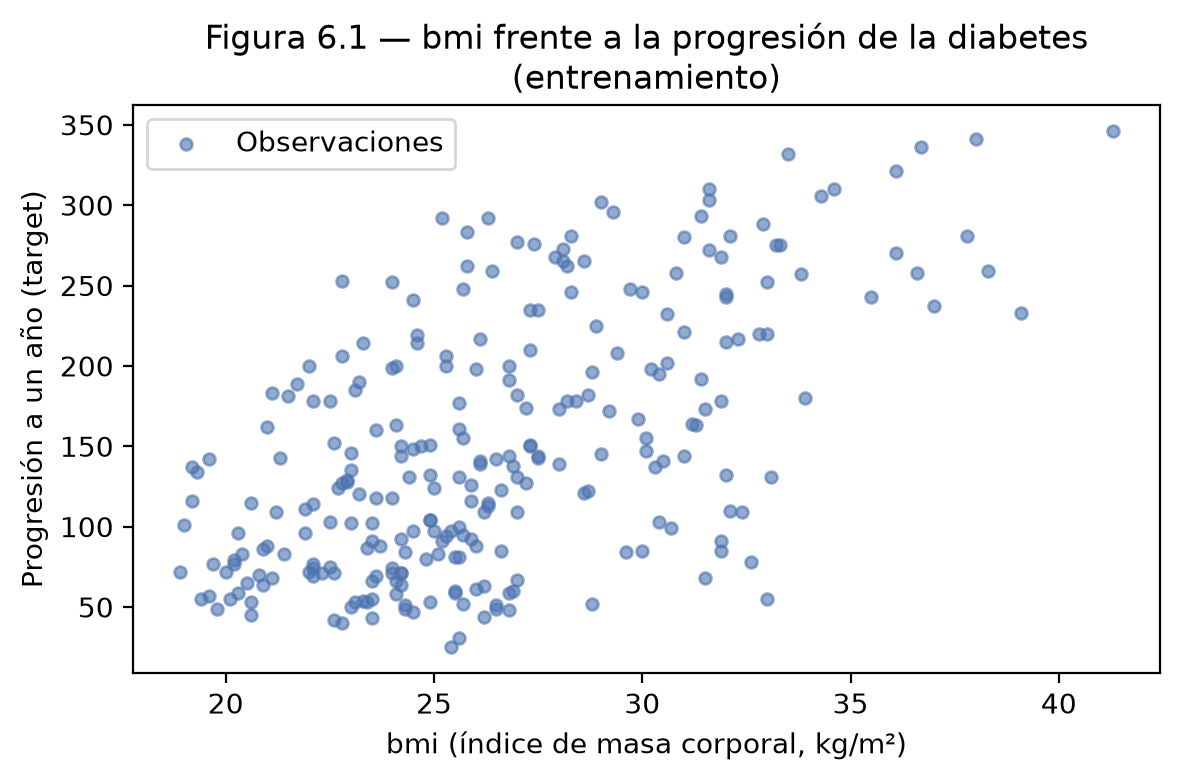
\includegraphics[width=0.68\textwidth]{figuras/ex6_bmi_target.png}
    \caption{\texttt{bmi} frente a la progresión de la diabetes (entrenamiento).}
    \label{fig:ex6-bmi}
\end{figure}

\item \textbf{Implementación con NumPy vs.\ \texttt{LinearRegression}.}
Aplicando a \texttt{bmi} las mismas expresiones que derivamos en el
Ejercicio~1 obtuvimos $\hat\beta_0 = \SimpleBetaCero$ y
$\hat\beta_1 = \SimpleBetaUno$, los mismos coeficientes que reporta
\texttt{LinearRegression}, y la diferencia absoluta máxima entre las
predicciones de validación de ambas implementaciones fue de
$\SimpleDifMax$, es decir, error de redondeo de punto flotante, por lo que
\texttt{np.allclose} devolvió \texttt{True}. Con esto nos quedó claro que,
con un solo predictor, scikit-learn resuelve exactamente el mismo problema
de mínimos cuadrados que hicimos a mano, solo que mediante una
factorización numérica en lugar de las sumas explícitas.

\item \textbf{Comparación con \texttt{DummyRegressor}.}

\begin{table}[H]
\centering
\small
% Archivo generado automáticamente por el notebook (no editar a mano).
\begin{tabular}{llrrr}
\toprule
Modelo & Partición & MAE & RMSE & $R^2$ \\
\midrule
Constante (media) & Entrenamiento & 66.6773 & 78.8462 & 0.0000 \\
Constante (media) & Validación & 64.1288 & 75.6392 & $-$0.0443 \\
Regresión simple (bmi) & Entrenamiento & 51.5459 & 63.3458 & 0.3545 \\
Regresión simple (bmi) & Validación & 50.3475 & 58.5671 & 0.3739 \\
\bottomrule
\end{tabular}

\caption{Predictor constante frente a regresión simple (entrenamiento y validación).}
\label{tab:ex6-comparacion}
\end{table}

La regresión simple mejoró las tres métricas frente al predictor constante
en ambas particiones (Tabla~\ref{tab:ex6-comparacion}): en validación el
RMSE bajó de $\RegDummyRMSEVal$ a $\RegSimpleRMSEVal$ y el MAE de
$\RegDummyMAEVal$ a $\RegSimpleMAEVal$, mientras que $R^2$ pasó de
$\RegDummyRdosVal$ a $\RegSimpleRdosVal$, de modo que \texttt{bmi} por sí
solo explica cerca de un tercio de la variabilidad en validación. El $R^2$
negativo de la constante al principio nos extrañó, pero no es un error: la
media se estima con entrenamiento y el $R^2$ de validación se mide contra la
media de validación, por lo que cualquier desfase entre ambas lo vuelve
ligeramente negativo, y en todo caso ninguna métrica empeoró con la
regresión simple. Algo que sí anotamos desde aquí es que los dos modelos
(incluida la constante) tuvieron menor error en validación que en
entrenamiento, lo que apunta a una partición de validación algo más
favorable y no a un fenómeno propio del modelo.

\item \textbf{Residuos de validación.}
Los residuos (Figura~\ref{fig:ex6-res}) se distribuyen alrededor de cero sin
una curvatura marcada, pero su dispersión crece con el valor predicho
(desviación estándar de $\ResStdBaja$ en la mitad de predicciones bajas
frente a $\ResStdAlta$ en la mitad alta), lo que nos hizo sospechar
heterocedasticidad, y hay errores grandes en ambos sentidos (entre $\ResMin$
y $\ResMax$). Esto implica que el RMSE resume un error que en realidad es
menor para pacientes con \texttt{bmi} bajo y mayor para \texttt{bmi} alto,
que los errores estándar clásicos de mínimos cuadrados (que suponen varianza
constante) no serían confiables para inferencia y que, con tanta dispersión
residual, faltan predictores. Eso fue lo que nos llevó al modelo múltiple
del Ejercicio~7.

\begin{figure}[H]
    \centering
    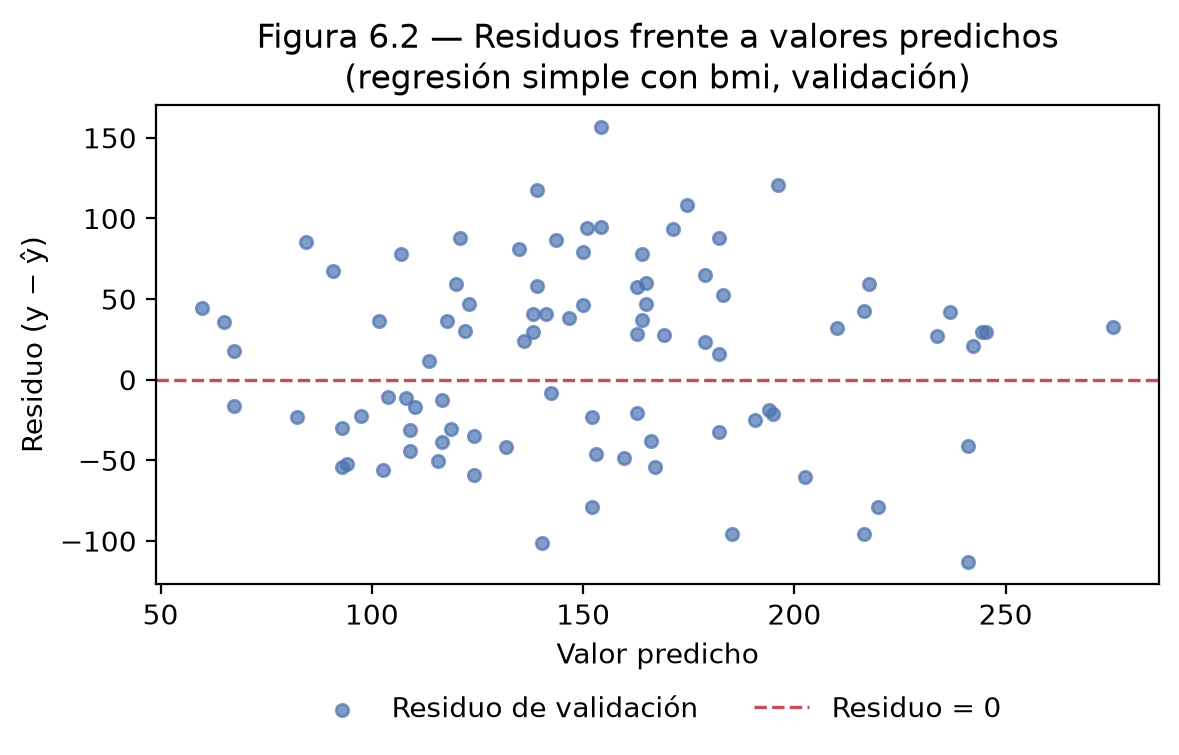
\includegraphics[width=0.68\textwidth]{figuras/ex6_residuos.png}
    \caption{Residuos frente a valores predichos de la regresión simple (validación).}
    \label{fig:ex6-res}
\end{figure}

\item \textbf{Interpretación de coeficientes y causalidad.}
El intercepto ($\SimpleBetaCero$) es la predicción para \texttt{bmi} igual
a cero, valor fuera del rango observado (Tabla~\ref{tab:ex6-exploracion}),
por lo que solo ubica la recta y no le dimos lectura práctica, mientras que
la pendiente ($\SimpleBetaUno$) indica que cada kg/m$^2$ adicional de
\texttt{bmi} se asocia, en promedio, con $\SimpleBetaUno$ unidades más de
progresión predicha. Esta asociación no identifica el efecto de intervenir
sobre \texttt{bmi}, pues los datos son observacionales y \texttt{bmi} se
relaciona con otros factores (presión arterial, lípidos, edad) que también
influyen en la progresión, de modo que la pendiente mezcla el efecto propio
de \texttt{bmi} con el de esas variables. De hecho, cuando pasamos al modelo
múltiple del Ejercicio~7 la pendiente equivalente bajó a unas
$\BmiPorUnidad$ unidades por kg/m$^2$.

\end{enumerate}

% =====================================================================
% ejercicio07.tex
% Responsabilidad única: ajustar la regresión múltiple estandarizada y la cuadrícula de árboles de
% regresión, y seleccionar con validación el candidato final de regresión.
% Las cifras provienen de generado/resultados.tex y generado/tabla_*.tex.
% =====================================================================
\subsection{Ejercicio 7 --- Caso A: regresión múltiple y árbol de regresión}

\begin{enumerate}

\item \textbf{Regresión múltiple con \texttt{Pipeline}.}
Se construyó un \texttt{Pipeline} con \texttt{StandardScaler} y
\texttt{LinearRegression}, de modo que medias y desviaciones se aprenden solo
con entrenamiento. El modelo múltiple obtuvo un RMSE de validación de
$\RegMultiRMSEVal$ (frente a $\RegSimpleRMSEVal$ del simple y
$\RegDummyRMSEVal$ de la constante) y un $R^2$ de validación de
$\RegMultiRdosVal$ (frente a $\RegSimpleRdosVal$), véase la
Tabla~\ref{tab:ex7-candidatos}. La mejora en entrenamiento (RMSE de
$\RegSimpleRMSETr$ a $\RegMultiRMSETr$) por sí sola no prueba nada, pues como
se justificó en el Ejercicio~2e añadir predictores nunca aumenta el error
mínimo de entrenamiento; lo relevante es que la mejora se conserva en
validación y que la brecha entre particiones no se abre.

\item \textbf{Coeficientes estandarizados y correlaciones.}
Cada coeficiente (Tabla~\ref{tab:ex7-coef}) es el cambio esperado en la
predicción ante un aumento de una desviación estándar de entrenamiento (la
poblacional que usa \texttt{StandardScaler}) en ese predictor, manteniendo
fijos los demás. Para \texttt{s5} un aumento de una desviación
($\DesvMultiScinco$ en el logaritmo de los triglicéridos) se asocia con
$\CoefMultiScinco$ unidades más de progresión, y para \texttt{bmi} un aumento
de una desviación ($\DesvMultiBmi$\,kg/m$^2$) se asocia con
$\CoefMultiBmi$ unidades más, equivalentes a unas $\BmiPorUnidad$ por
kg/m$^2$, cerca de la mitad de la pendiente simple ($\SimpleBetaUno$), ya que
allí \texttt{bmi} absorbía parte de lo que ahora explican predictores
correlacionados con él.

\begin{table}[H]
\centering
\small
% Archivo generado automáticamente por el notebook (no editar a mano).
\begin{tabular}{lrrr}
\toprule
Predictor & Coeficiente & Desv. est. (ent.) & Corr. con $y$ (ent.) \\
\midrule
s1 & $-$51.1014 & 35.2232 & 0.1623 \\
s5 & 37.2716 & 0.5015 & 0.5645 \\
s2 & 27.4808 & 31.2424 & 0.1073 \\
bmi & 25.0766 & 4.3741 & 0.5954 \\
bp & 15.1673 & 14.0075 & 0.4197 \\
s4 & 15.0321 & 1.2713 & 0.4076 \\
sex & $-$11.3593 & 0.4999 & $-$0.0275 \\
s3 & 10.8403 & 12.2802 & $-$0.3798 \\
s6 & 3.8171 & 11.4005 & 0.3867 \\
age & 1.1318 & 12.7451 & 0.2061 \\
\bottomrule
\end{tabular}

\caption{Coeficientes estandarizados de la regresión múltiple, ordenados por magnitud absoluta (entrenamiento).}
\label{tab:ex7-coef}
\end{table}

La matriz de correlaciones (Figura~\ref{fig:ex7-corr}) muestra pares
fuertemente relacionados, en especial \texttt{s1} y \texttt{s2}
($\CorrSunoSdos$) y \texttt{s3} y \texttt{s4} ($\CorrStresScuatro$). El caso
de \texttt{s1} y \texttt{s2} ilustra el problema, pues ambos tienen
correlación positiva con la variable objetivo ($\CorrYSuno$ y $\CorrYSdos$),
pero el modelo les asigna coeficientes de signo opuesto y gran magnitud
($\CoefMultiSuno$ y $\CoefMultiSdos$), porque al moverse casi juntos el
ajuste aprovecha su diferencia y no el nivel de cada uno; algo similar ocurre
con \texttt{s3}, de correlación negativa con el \emph{target}
($\CorrYStres$) y coeficiente positivo ($\CoefMultiStres$). Por esto los
coeficientes deben leerse como efectos parciales condicionados al resto,
inestables ante colinealidad, y no como importancias independientes.

\begin{figure}[H]
    \centering
    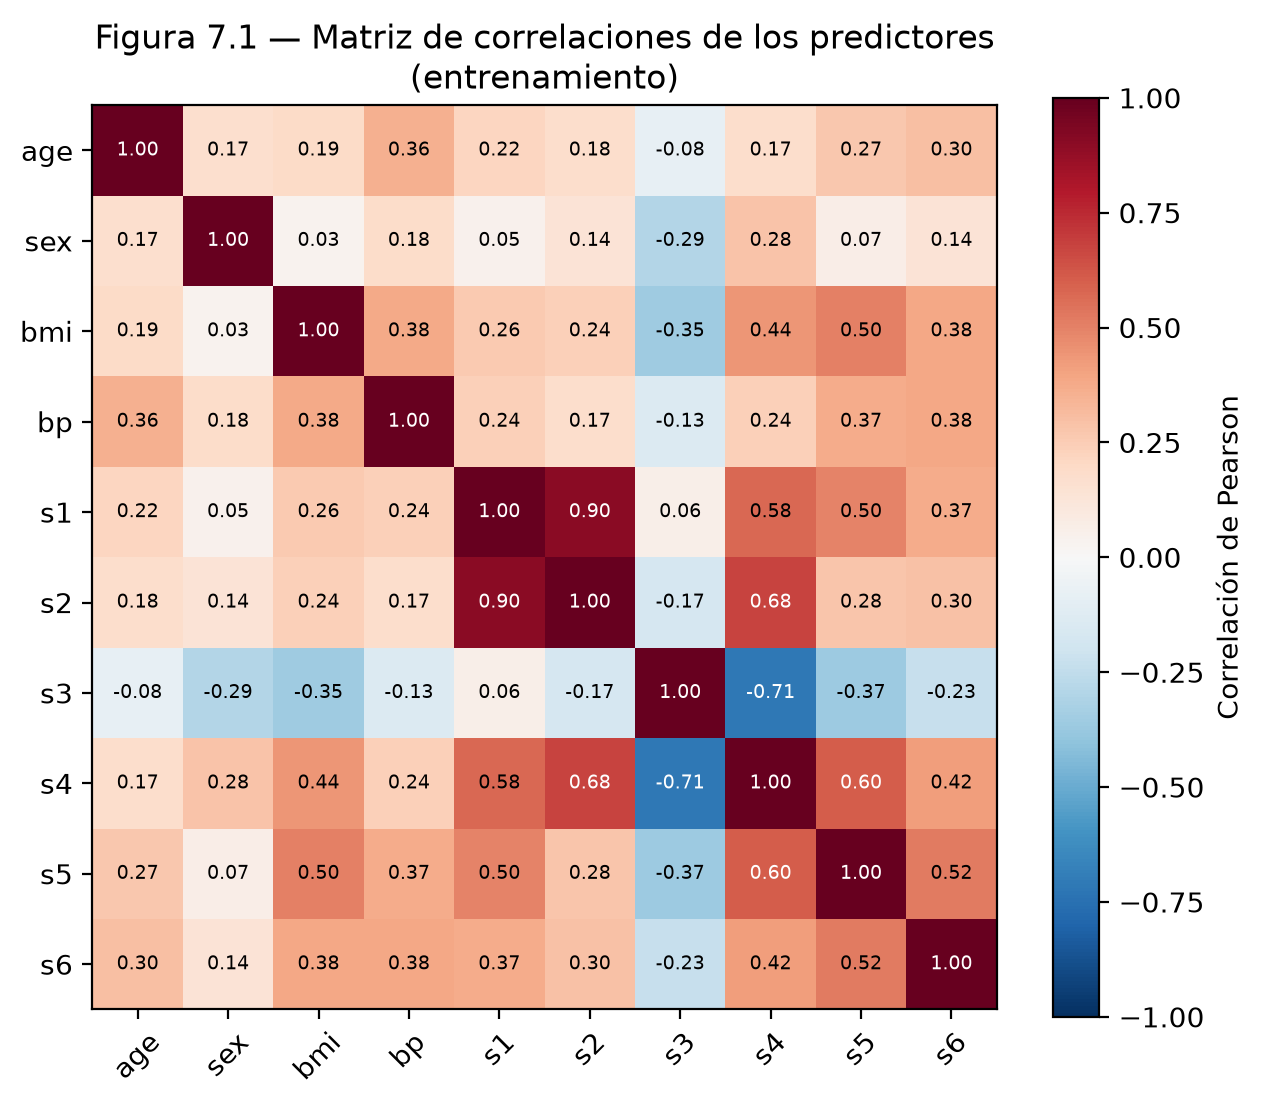
\includegraphics[width=0.62\textwidth]{figuras/ex7_correlaciones.png}
    \caption{Matriz de correlaciones de los predictores (entrenamiento).}
    \label{fig:ex7-corr}
\end{figure}

\item \textbf{Cuadrícula de \texttt{DecisionTreeRegressor}.}

\begin{table}[H]
\centering
\small
% Archivo generado automáticamente por el notebook (no editar a mano).
\begin{tabular}{rrrrrrr}
\toprule
max\_depth & min\_samples\_leaf & RMSE ent. & RMSE val. & Prof. real & Hojas & Brecha \\
\midrule
2 & 5 & 57.6273 & 58.7814 & 2 & 4 & 1.1541 \\
2 & 15 & 57.6273 & 58.7814 & 2 & 4 & 1.1541 \\
2 & 30 & 59.0808 & 57.3406 & 2 & 4 & $-$1.7402 \\
4 & 5 & 49.0068 & 61.0539 & 4 & 15 & 12.0471 \\
4 & 15 & 52.7463 & 58.1889 & 4 & 10 & 5.4425 \\
4 & 30 & 58.0732 & 56.7789 & 4 & 6 & $-$1.2943 \\
6 & 5 & 38.5411 & 63.2140 & 6 & 31 & 24.6729 \\
6 & 15 & 52.1941 & 57.9781 & 6 & 12 & 5.7840 \\
6 & 30 & 58.0732 & 56.7789 & 4 & 6 & $-$1.2943 \\
\bottomrule
\end{tabular}

\caption{Árboles de regresión: RMSE de entrenamiento y validación, profundidad real y hojas.}
\label{tab:ex7-arboles}
\end{table}

Con \texttt{min\_samples\_leaf} $=5$ aparece el patrón clásico de
sobreajuste (Tabla~\ref{tab:ex7-arboles}), al aumentar la profundidad el
RMSE de entrenamiento baja y el de validación sube, hasta
$\ArbolProfundoRMSETr$ frente a $\ArbolProfundoRMSEVal$ con
$\ArbolProfundoHojas$ hojas en profundidad 6. Con \texttt{min\_samples\_leaf}
$=30$ domina la restricción de tamaño de hoja, de forma que con
\texttt{max\_depth} $=6$ el árbol no supera la profundidad real 4 y resulta
idéntico al de \texttt{max\_depth} $=4$ (hay $\ArbolRegEmpatados$ árboles con
el mismo RMSE de validación mínimo, $\ArbolRegRMSEVal$); ante ese empate la
regla elige la menor profundidad máxima, es decir
\texttt{max\_depth} $=\ArbolRegMaxDepth$ y \texttt{min\_samples\_leaf}
$=\ArbolRegMinLeaf$, con profundidad real $\ArbolRegProf$ y $\ArbolRegHojas$
hojas.

\item \textbf{Candidato final de regresión.}

\begin{table}[H]
\centering
\resizebox{\textwidth}{!}{% Archivo generado automáticamente por el notebook (no editar a mano).
\begin{tabular}{lrrrrrr}
\toprule
Modelo & MAE ent. & RMSE ent. & $R^2$ ent. & MAE val. & RMSE val. & $R^2$ val. \\
\midrule
Regresión simple (bmi) & 51.5459 & 63.3458 & 0.3545 & 50.3475 & 58.5671 & 0.3739 \\
Regresión múltiple (10 predictores) & 43.7935 & 54.6104 & 0.5203 & 42.9389 & 51.1937 & 0.5216 \\
Árbol (max\_depth=4, min\_samples\_leaf=30) & 46.5549 & 58.0732 & 0.4575 & 45.3006 & 56.7789 & 0.4116 \\
Constante (media) — referencia & 66.6773 & 78.8462 & 0.0000 & 64.1288 & 75.6392 & $-$0.0443 \\
\bottomrule
\end{tabular}
}
\caption{Candidatos de regresión y referencia constante (entrenamiento y validación).}
\label{tab:ex7-candidatos}
\end{table}

El candidato final de regresión es la \textbf{regresión múltiple}, con el
menor RMSE de validación ($\CandidatoRegRMSEVal$), por delante del árbol
seleccionado ($\ArbolRegRMSEVal$) y del modelo simple ($\RegSimpleRMSEVal$),
sin necesidad de aplicar la regla de desempate; la constante
($\RegDummyRMSEVal$) queda como referencia. La decisión se congeló antes de
consultar la prueba.

\item \textbf{No linealidad del árbol y brecha entrenamiento--validación.}
El árbol divide el espacio con umbrales sobre los valores originales, de
modo que solo importa el orden de los valores y no su escala (por eso no
necesita estandarización), y al asignar una constante por región puede
representar relaciones no lineales e interacciones sin especificarlas. Sin
embargo, esa flexibilidad no garantiza superar al modelo múltiple, pues con
$\NRegTr$ observaciones de entrenamiento y un mínimo de $\ArbolRegMinLeaf$
por hoja el árbol seleccionado solo produce $\ArbolRegHojas$ valores
distintos de predicción, una aproximación escalonada de una relación que
aquí parece mayormente aditiva y cercana a lineal. El árbol seleccionado
tiene una brecha pequeña ($\ArbolRegRMSETr$ en entrenamiento y
$\ArbolRegRMSEVal$ en validación), pero su error supera al del modelo múltiple
en ambas particiones, y el árbol profundo descrito en el inciso c muestra que
la flexibilidad adicional se traduce en memorizar el entrenamiento y no en
generalizar mejor.

\end{enumerate}

% =====================================================================
% ejercicio08.tex
% Responsabilidad única: ajustar la regresión logística regularizada en el caso cáncer de mama,
% seleccionar $C$ por ROC-AUC de validación y fijar el umbral por costo.
% Las cifras provienen de generado/resultados.tex y generado/tabla_*.tex.
% =====================================================================
\subsection{Ejercicio 8: Caso B, regresión logística y elección del umbral}

\paragraph{Qué buscamos.} Pasamos al caso del cáncer de mama, donde hay
que decidir si una muestra es maligna. Usamos la regresión logística de
los ejercicios 3 y 4, ahora con los $30$ predictores estandarizados. Hay
dos decisiones que tomar con validación y en este orden: primero cuánto
regularizar (el hiperparámetro $C$), lo que fija el modelo y sus
probabilidades, y después a partir de qué probabilidad declaramos una
muestra como maligna (el umbral $t$), lo que convierte probabilidades en
decisiones.

\begin{enumerate}

\item \textbf{Particiones, recodificación y referencia.}
Antes de ajustar nada quisimos estar seguros de la recodificación, así que
hicimos una tabla cruzada (un conteo de cuántas muestras hay en cada
combinación de etiqueta original y etiqueta nueva): los 212 tumores
\texttt{malignant} quedaron con $y=1$ y los 357 \texttt{benign} con
$y=0$, de modo que las métricas de la clase positiva hablan de muestras
malignas. La proporción de malignos fue $\PropMalTr$ en entrenamiento y
$\PropMalVal$ en validación, prácticamente iguales gracias a la
estratificación.

Como referencia usamos \texttt{DummyClassifier} con
\texttt{strategy="prior"}, que le asigna a todas las muestras la misma
probabilidad de maligno, la proporción de entrenamiento ($\PropMalTr$).
Como esa probabilidad es menor que $0.5$, con $t=0.5$ predice siempre
benigno: no tiene verdaderos ni falsos positivos. Su precisión,
$TP/(TP+FP)=0/0$, queda indefinida, y el argumento \texttt{zero\_division=0}
le dice a scikit-learn que la reporte como 0, al igual que el recall
($0$ malignos detectados) y el F1. Su ROC-AUC es exactamente $0.5$: como da
el mismo puntaje a todas las muestras, no pone ningún maligno por encima
de ningún benigno, y eso es lo mismo que ordenar al azar.

\item \textbf{Selección de $C$.}
Probamos $C\in\{0.01,\,0.1,\,1,\,10\}$, de mucha a poca regularización
(recordemos del Ejercicio~4e que un $C$ pequeño castiga más los
coeficientes). Como criterio usamos el ROC-AUC de validación porque no
depende del umbral, que todavía no habíamos elegido: mide qué tan bien el
modelo \emph{ordena} las muestras, poniendo las malignas por encima de las
benignas.

\begin{table}[H]
\centering
\resizebox{\textwidth}{!}{% Archivo generado automáticamente por el notebook (no editar a mano).
\begin{tabular}{lrrrrrl}
\toprule
C & ROC-AUC ent. & ROC-AUC val. & F1 ent. (t=0.5) & F1 val. (t=0.5) & Iteraciones & Convergió \\
\midrule
0.01 & 0.9927 & 0.9905 & 0.9283 & 0.9512 & 10 & Sí \\
0.1 & 0.9955 & 0.9951 & 0.9721 & 0.9762 & 10 & Sí \\
1 & 0.9979 & 0.9957 & 0.9840 & 0.9655 & 18 & Sí \\
10 & 0.9997 & 0.9957 & 0.9960 & 0.9545 & 33 & Sí \\
\bottomrule
\end{tabular}
}
\caption{Regresión logística según $C$: ROC-AUC y F1 ($t=0.5$) en entrenamiento y validación, y convergencia.}
\label{tab:ex8-C}
\end{table}

El ajuste usa el algoritmo \texttt{lbfgs}, que, como el descenso de
gradiente del Ejercicio~4c, mejora los coeficientes paso a paso hasta que
los cambios son despreciables. Decimos que \emph{convergió} si llegó a ese
punto antes del límite de pasos que le fijamos. Los cuatro ajustes
convergieron (como máximo $\LogitIterMax$ iteraciones, lejos del límite de
5000, y sin la advertencia \texttt{ConvergenceWarning}).

El ROC-AUC de validación creció con $C$ hasta estabilizarse
(Tabla~\ref{tab:ex8-C}), y nos encontramos con que $\LogitEmpatesC$
valores de $C$ ($C=1$ y $C=10$) obtuvieron exactamente el mismo máximo a
precisión completa (que redondeado es $\LogitAUCVal$). Al principio nos
pareció raro, pero tiene explicación: el AUC es la fracción de parejas
(maligno, benigno) de validación en las que el maligno recibe mayor
probabilidad, y con $\NClfVal$ muestras es un cociente de números enteros;
si dos modelos ordenan bien exactamente las mismas parejas, empatan. Ante
ese empate nuestra regla fue elegir el menor, $\boldsymbol{C=\LogitC}$,
el de mayor regularización entre los empatados (el más sencillo).

En entrenamiento el ROC-AUC y el F1 aumentan con $C$, como era de esperar
al soltar la regularización, mientras que el F1 de validación alcanzó su
máximo en $C=0.1$ y cayó en $C=10$: con menos regularización el modelo se
ajusta más al entrenamiento sin ganar en datos nuevos. Aun así no elegimos
$C=0.1$ pese a tener el mejor F1 con umbral 0.5, porque el criterio que
fijamos de antemano fue el ROC-AUC y el F1 depende de un umbral que aún no
estaba decidido.

\item \textbf{Umbral por costo $L = FP + 5FN$.}
Con el modelo ya fijo, recorrimos los umbrales
$t\in\{0.2,0.3,\dots,0.8\}$ y para cada uno contamos en validación los
falsos positivos y falsos negativos y el costo $L=FP+5FN$ del enunciado,
que pesa cinco veces más dejar escapar un maligno que dar una falsa
alarma. Las reglas para elegir, en orden, fueron: menor costo; si hay
empate, mayor recall; y si sigue el empate, menor umbral.

\begin{table}[H]
\centering
\small
% Archivo generado automáticamente por el notebook (no editar a mano).
\begin{tabular}{lrrrrrr}
\toprule
Umbral & Precisión & Recall & F1 & FP & FN & Costo L \\
\midrule
0.2 & 0.8400 & 0.9767 & 0.9032 & 8 & 1 & 13 \\
0.3 & 0.9130 & 0.9767 & 0.9438 & 4 & 1 & 9 \\
0.4 & 0.9545 & 0.9767 & 0.9655 & 2 & 1 & 7 \\
0.5 & 0.9545 & 0.9767 & 0.9655 & 2 & 1 & 7 \\
0.6 & 0.9545 & 0.9767 & 0.9655 & 2 & 1 & 7 \\
0.7 & 1.0000 & 0.9767 & 0.9882 & 0 & 1 & 5 \\
0.8 & 1.0000 & 0.9767 & 0.9882 & 0 & 1 & 5 \\
\bottomrule
\end{tabular}

\caption{Umbrales para la regresión logística con $C=\LogitC$ (validación).}
\label{tab:ex8-umbrales}
\end{table}

El costo bajó al subir el umbral (Tabla~\ref{tab:ex8-umbrales}) y alcanzó
su mínimo, $L=\LogitCostoSel$ ($FP=\LogitFPSel$, $FN=\LogitFNSel$), en
$t=0.7$ y $t=0.8$. Como ambos tienen el mismo recall ($\LogitRecallSel$),
el último desempate eligió el menor umbral, $\boldsymbol{t=\LogitT}$.
Frente a $t=0.5$ ($L=\LogitCostoMedio$, con $FP=\LogitFPMedio$ y
$FN=\LogitFNMedio$), el umbral elegido elimina las falsas alarmas sin
perder ningún maligno adicional.

Eso sí, aquí nos quedó una duda que vale la pena dejar escrita. El recall
es igual en los siete umbrales porque el único maligno que el modelo no
detecta tiene probabilidad menor que $0.2$, así que en validación subir el
umbral solo quita falsos positivos y nunca agrega falsos negativos. Pero
con probabilidades bien calibradas, el razonamiento del Ejercicio~3d daría
para esta razón de costos un umbral teórico de $1/(1+5)\approx0.167$, muy
por debajo de $\LogitT$. Es decir, la elección de un umbral alto descansa
en unos pocos casos de validación, y en datos nuevos podrían aparecer
malignos con probabilidades intermedias que este umbral deje pasar.

\item \textbf{Precisión y recall frente al umbral.}
En la Figura~\ref{fig:ex8-pr}, al subir el umbral la precisión aumenta:
exigimos una probabilidad más alta para declarar maligno, así que
descartamos falsos positivos y los que quedan marcados son más seguros. El
recall se mantuvo constante por lo que explicamos en el inciso anterior;
en general bajaría, porque un umbral más exigente termina dejando pasar
malignos. Ese es el tira y afloje entre precisión y recall que el umbral
regula.

El ROC-AUC ($\LogitAUCVal$), en cambio, no cambia con $t$. La curva ROC
dibuja, para \emph{todos} los umbrales posibles, la fracción de malignos
detectados contra la fracción de benignos marcados por error, y el AUC es
el área bajo esa curva; elegir $t$ solo escoge un punto de la curva. Por
eso usamos el ROC-AUC para comparar modelos (valores de $C$) sin importar
el punto de operación, y el costo $L$ para fijar, una vez congelado el
modelo, el umbral que mejor equilibra falsos positivos y falsos negativos
según sus consecuencias.

\begin{figure}[H]
    \centering
    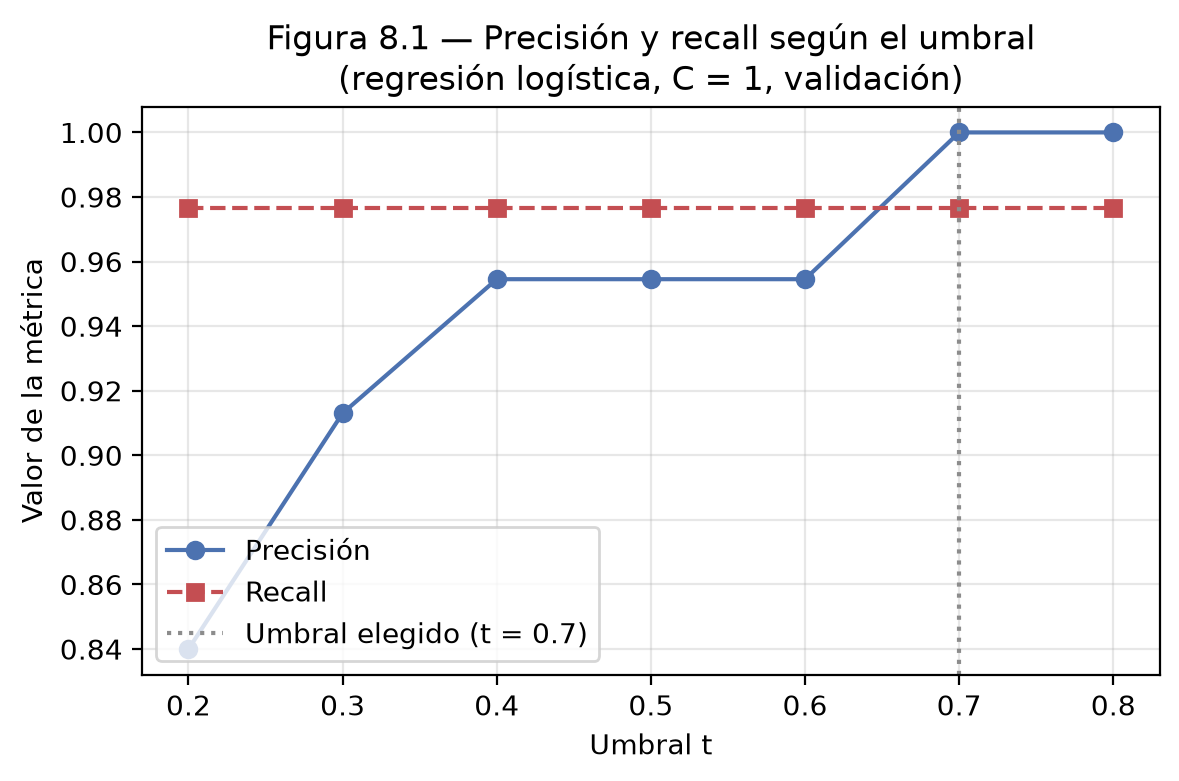
\includegraphics[width=0.68\textwidth]{figuras/ex8_precision_recall.png}
    \caption{Precisión y recall según el umbral, regresión logística con $C=\LogitC$ (validación).}
    \label{fig:ex8-pr}
\end{figure}

\item \textbf{Coeficientes estandarizados y odds.}
Recordemos del Ejercicio~3a que la regresión logística es lineal en los
log-odds: $\log\frac{p}{1-p}=\beta_0+\beta_1z_1+\dots+\beta_{30}z_{30}$, con
las $z$ estandarizadas. Así, cada coeficiente es lo que suben los
log-odds de malignidad cuando ese predictor aumenta una desviación
estándar de entrenamiento y los demás quedan fijos.

\begin{table}[H]
\centering
\small
% Archivo generado automáticamente por el notebook (no editar a mano).
\begin{tabular}{lrr}
\toprule
Predictor & Coeficiente & $e^{\beta}$ \\
\midrule
worst texture & 1.3553 & 3.8780 \\
mean concave points & 1.1043 & 3.0171 \\
radius error & 1.0259 & 2.7897 \\
worst symmetry & 0.9519 & 2.5905 \\
worst radius & 0.8134 & 2.2556 \\
worst area & 0.7948 & 2.2140 \\
area error & 0.7822 & 2.1864 \\
worst concavity & 0.7689 & 2.1575 \\
mean concavity & 0.7621 & 2.1428 \\
compactness error & $-$0.7591 & 0.4681 \\
\bottomrule
\end{tabular}

\caption{Diez mayores coeficientes estandarizados (en magnitud) de la regresión logística con $C=\LogitC$.}
\label{tab:ex8-coef}
\end{table}

Un coeficiente positivo indica que valores más altos del predictor se
asocian con mayor probabilidad de malignidad, y uno negativo lo contrario.
\texttt{worst texture} ($\CoefTexturaPeor$) y \texttt{mean concave points}
($\CoefPuntosConcavos$) salieron con signo positivo, coherente con que
núcleos de textura más irregular y con más hundimientos en el borde se
asocien con malignidad. En cambio \texttt{compactness error}
($\CoefCompactError$) salió con signo negativo, y nos tocó tener cuidado
al leerlo: no significa que valores altos de esa variable, por sí solos,
indiquen benignidad, sino que es un efecto condicional al resto de las 29
variables, muchas de ellas casi repetidas entre sí (radio, perímetro y área
miden casi lo mismo), y ya vimos en el Ejercicio~7 que en ese caso los
signos individuales pierden lectura.

Para pasar a odds se usa el factor $e^{\beta}$ del Ejercicio~3a. Para
\texttt{worst texture}, $e^{\CoefTexturaPeor}\approx\ExpTexturaPeor$: subir
una desviación estándar de entrenamiento multiplica los odds estimados de
malignidad por cerca de $\ExpTexturaPeor$, con las demás variables fijas.
Esto describe una asociación dentro del modelo y no un efecto causal. Con
esto dejamos congelados el pipeline con $C=\LogitC$ y el umbral
$t=\LogitT$.

\end{enumerate}

% =====================================================================
% ejercicio09.tex
% Responsabilidad única: ajustar la cuadrícula de árboles de clasificación, elegir árbol y umbral
% con validación, comparar con la logística e interpretar reglas e
% importancias.
% Las cifras provienen de generado/resultados.tex y generado/tabla_*.tex.
% =====================================================================
\subsection{Ejercicio 9: Caso B, árbol de clasificación e interpretación}

\paragraph{Qué buscamos.} Para el mismo problema del cáncer de mama
probamos ahora un árbol de clasificación, el modelo del Ejercicio~5a: hace
preguntas sobre las variables y cada hoja da como probabilidad de maligno
la proporción de malignos que cayeron en ella. Su atractivo es que se puede
leer como un conjunto de reglas. Elegimos el árbol y su umbral con
validación, lo comparamos con la regresión logística del Ejercicio~8 y
miramos qué variables usa.

\begin{enumerate}

\item \textbf{Cuadrícula de \texttt{DecisionTreeClassifier}.}
Ajustamos doce árboles, todas las combinaciones de
\texttt{max\_depth} $\in\{2,3,5,\texttt{None}\}$ (\texttt{None} significa sin
límite de profundidad) y \texttt{min\_samples\_leaf} $\in\{1,5,15\}$, con el
criterio de Gini del Ejercicio~5a para elegir las preguntas y
\texttt{random\_state=42} para que los resultados se puedan repetir.
Usamos los predictores originales sin estandarizar, porque a un árbol solo
le importa si un valor está por encima o por debajo de un corte, no su
escala. Recorrimos la cuadrícula con \texttt{max\_depth} por fuera y
\texttt{min\_samples\_leaf} por dentro, y ese orden quedó como último
criterio de desempate.

Nos dimos cuenta de que \texttt{min\_samples\_leaf} limita por sí solo la
profundidad: con hojas de al menos 5 o 15 muestras, los árboles con
\texttt{max\_depth} igual a 5 y a \texttt{None} resultaron idénticos
(Tabla~\ref{tab:ex9-arboles}), porque antes de llegar a profundidad 5 ya no
quedan grupos lo bastante grandes para partir. En el otro extremo, el árbol
sin ninguna restricción alcanzó ROC-AUC y F1 de entrenamiento de
$\ArbolLibreAUCTr$, es decir, clasificó perfecto el entrenamiento: señal de
que lo memorizó.

\item \textbf{Selección del árbol.}
Como en el Ejercicio~8, elegimos con el ROC-AUC de validación porque no
depende del umbral. El F1 de la tabla usa la regla
$\hat y=\mathbf{1}[p\ge0.5]$, que se lee \emph{predecir $1$ si $p\ge0.5$ y
$0$ si no}.

\begin{table}[H]
\centering
\resizebox{\textwidth}{!}{% Archivo generado automáticamente por el notebook (no editar a mano).
\begin{tabular}{lrrrrrrr}
\toprule
max\_depth & min\_samples\_leaf & ROC-AUC ent. & ROC-AUC val. & F1 ent. & F1 val. & Prof. real & Hojas \\
\midrule
2 & 1 & 0.9726 & 0.9492 & 0.9308 & 0.8571 & 2 & 4 \\
2 & 5 & 0.9726 & 0.9492 & 0.9308 & 0.8571 & 2 & 4 \\
2 & 15 & 0.9754 & 0.9656 & 0.9213 & 0.8817 & 2 & 4 \\
3 & 1 & 0.9893 & 0.8898 & 0.9762 & 0.8941 & 3 & 8 \\
3 & 5 & 0.9928 & 0.9589 & 0.9600 & 0.8941 & 3 & 7 \\
3 & 15 & 0.9854 & 0.9745 & 0.9213 & 0.8817 & 3 & 5 \\
5 & 1 & 0.9999 & 0.9270 & 0.9960 & 0.9091 & 5 & 16 \\
5 & 5 & 0.9976 & 0.9466 & 0.9647 & 0.8864 & 4 & 10 \\
5 & 15 & 0.9886 & 0.9735 & 0.9213 & 0.8817 & 4 & 6 \\
None & 1 & 1.0000 & 0.9042 & 1.0000 & 0.8764 & 6 & 17 \\
None & 5 & 0.9976 & 0.9466 & 0.9647 & 0.8864 & 4 & 10 \\
None & 15 & 0.9886 & 0.9735 & 0.9213 & 0.8817 & 4 & 6 \\
\bottomrule
\end{tabular}
}
\caption{Árboles de clasificación: ROC-AUC y F1 ($\hat y = \mathbf{1}[p\ge 0.5]$) en entrenamiento y validación.}
\label{tab:ex9-arboles}
\end{table}

Seleccionamos el árbol de \texttt{max\_depth} $=\ArbolClfMaxDepth$ y
\texttt{min\_samples\_leaf} $=\ArbolClfMinLeaf$, que tuvo el mayor ROC-AUC
de validación ($\ArbolClfAUCVal$), con profundidad real $\ArbolClfProf$ y
$\ArbolClfHojas$ hojas. Su máximo es único (una sola fila lo alcanza), así
que esta vez no hubo que desempatar. Los árboles con hojas de una sola
muestra y profundidad real de 3 o más quedaron entre los peores en
validación pese a tener los mejores valores de entrenamiento, el mismo
patrón de sobreajuste del Ejercicio~7.

\item \textbf{Umbral del árbol y candidato final de clasificación.}
Repetimos el procedimiento del Ejercicio~8c con los mismos siete umbrales
y las mismas reglas (menor costo, luego mayor recall, luego menor umbral).

\begin{table}[H]
\centering
\small
% Archivo generado automáticamente por el notebook (no editar a mano).
\begin{tabular}{lrrrrrr}
\toprule
Umbral & Precisión & Recall & F1 & FP & FN & Costo L \\
\midrule
0.2 & 0.7636 & 0.9767 & 0.8571 & 13 & 1 & 18 \\
0.3 & 0.8200 & 0.9535 & 0.8817 & 9 & 2 & 19 \\
0.4 & 0.8200 & 0.9535 & 0.8817 & 9 & 2 & 19 \\
0.5 & 0.8200 & 0.9535 & 0.8817 & 9 & 2 & 19 \\
0.6 & 0.9487 & 0.8605 & 0.9024 & 2 & 6 & 32 \\
0.7 & 1.0000 & 0.7907 & 0.8831 & 0 & 9 & 45 \\
0.8 & 1.0000 & 0.7907 & 0.8831 & 0 & 9 & 45 \\
\bottomrule
\end{tabular}

\caption{Umbrales para el árbol seleccionado (validación).}
\label{tab:ex9-umbrales}
\end{table}

Al ver la Tabla~\ref{tab:ex9-umbrales} nos llamó la atención que varias
filas coincidieran, y la razón es la del Ejercicio~5b: el árbol solo puede
dar tantas probabilidades distintas como hojas tiene (la proporción de
malignos de cada hoja), así que todos los umbrales que caen entre dos de
esos valores producen exactamente las mismas predicciones. El menor costo
lo obtuvimos con $\boldsymbol{t=\ArbolT}$ ($L=\ArbolCostoSel$, con
$FP=\ArbolFPSel$ y $FN=\ArbolFNSel$), donde la regla $p\ge t$ incluye la hoja
cuya proporción de malignos es exactamente 0.2.

Para elegir el candidato final de clasificación entre la logística y el
árbol comparamos sus costos de validación (en empate habríamos mirado el
ROC-AUC). El costo del árbol es claramente mayor que el de la regresión
logística ($L=\LogitCostoSel$), por lo que nos quedamos con la
\textbf{regresión logística con $C=\LogitC$ y $t=\LogitT$}, sin necesidad de
desempates; su ROC-AUC de validación también es mayor ($\LogitAUCVal$
frente a $\ArbolClfAUCVal$).

\paragraph{Puente con el Ejercicio~3d: umbral teórico y calibración.}
En el Ejercicio~3d demostramos que, si las probabilidades están bien
calibradas, el umbral de costo mínimo es $t^*=c_{FP}/(c_{FP}+c_{FN})$, que
para $L=FP+5FN$ (es decir, $c_{FP}=1$ y $c_{FN}=5$) vale
$t^*=1/6\approx\TTeorico$. Nos pareció que valía la pena contrastar esa
predicción de la teoría con lo que elegimos en la práctica
(Tabla~\ref{tab:ex9-puente} y Figura~\ref{fig:ex9-calibracion}). El
contraste es solo descriptivo: el enunciado fija la rejilla de siete
umbrales, así que $t^*$ no lo usamos para seleccionar ni cambia ningún
candidato.

Para revisar la calibración usamos dos herramientas. La \emph{curva de
calibración} ordena las muestras de validación por su probabilidad
predicha, las reparte en cinco grupos de igual tamaño y, para cada grupo,
compara la probabilidad predicha promedio con la fracción de malignos que
de verdad hay en él; si el modelo está bien calibrado, los puntos caen
sobre la diagonal. El \emph{puntaje de Brier} (Tabla~\ref{tab:metricas})
resume en un número qué tan cerca están las probabilidades de lo que
ocurrió.

\begin{table}[H]
\centering
\small
% Archivo generado automáticamente por el notebook (no editar a mano).
\begin{tabular}{lrlrrrr}
\toprule
Modelo & Brier & t elegido & L (t elegido) & L (t* = 1/6) & FP (t*) & FN (t*) \\
\midrule
Regresión logística & 0.0201 & 0.7 & 5 & 15 & 10 & 1 \\
Árbol & 0.0528 & 0.2 & 18 & 18 & 13 & 1 \\
\bottomrule
\end{tabular}

\caption{Umbral teórico $t^*=1/6$ del Ejercicio~3d frente al umbral
elegido, y puntaje de Brier (validación).}
\label{tab:ex9-puente}
\end{table}

\begin{figure}[H]
    \centering
    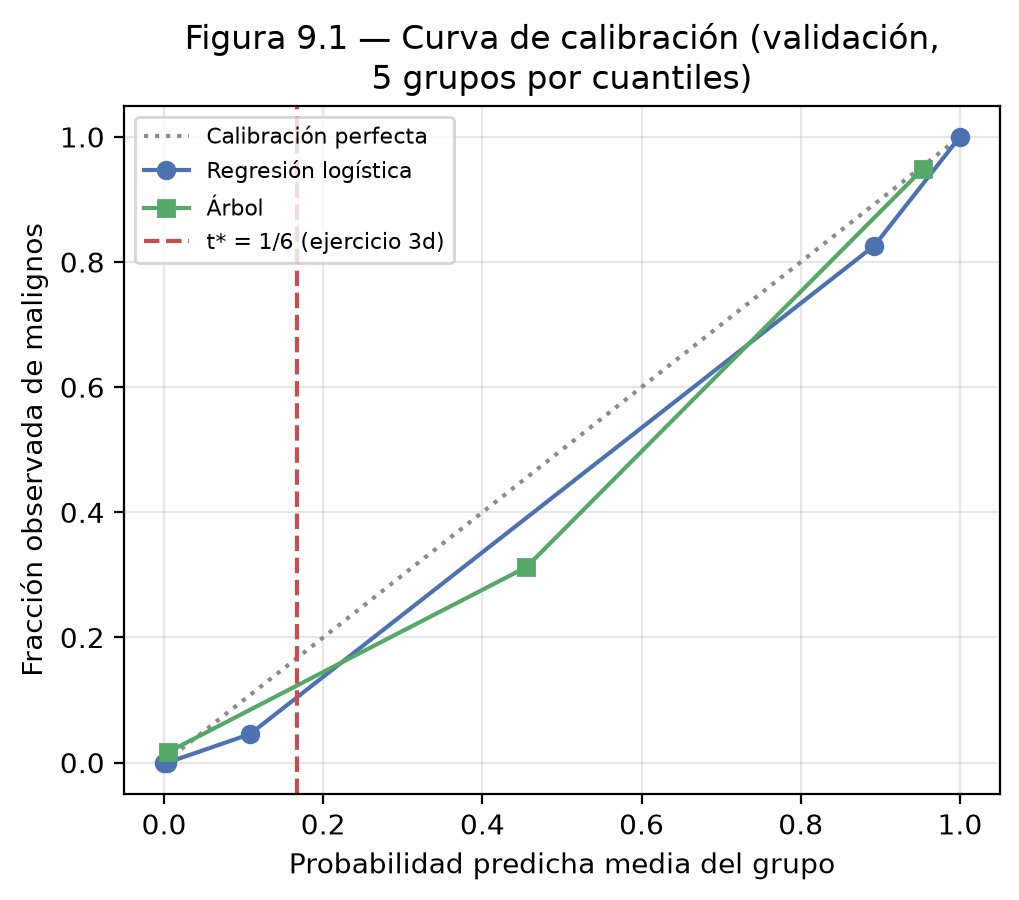
\includegraphics[width=0.6\textwidth]{figuras/ex9_calibracion.png}
    \caption{Curva de calibración en validación (cinco grupos por
    cuantiles): fracción observada de malignos frente a la probabilidad
    predicha media de cada grupo, con $t^*=1/6$ marcado en rojo.}
    \label{fig:ex9-calibracion}
\end{figure}

En el árbol la teoría y la práctica coincidieron, pues $t^*$ produce
exactamente las mismas predicciones que $t=\ArbolT$ ($L=\ArbolCostoTeo$):
ninguna hoja tiene una probabilidad entre $\TTeorico$ y $0.2$, y $0.2$ es
el valor de la rejilla más cercano a $t^*$. En la regresión logística, en
cambio, $t^*$ daría $L=\LogitCostoTeo$ ($FP=\LogitFPTeo$, $FN=\LogitFNTeo$),
el triple que el umbral elegido, y le dimos varias vueltas hasta ver que
la diferencia se explica por las condiciones que exige el resultado
teórico:
\begin{itemize}
    \item \textbf{La calibración no es perfecta.} En el grupo de
    probabilidades bajas (probabilidad predicha media de $\LogitCalMedia$)
    la fracción real de malignos es solo $\LogitCalFrac$. O sea, en esa
    zona el modelo exagera el riesgo, justo donde cae $t^*$, y bajar el
    umbral hasta allí agrega falsos positivos que en realidad son
    benignos.
    \item \textbf{Un caso puntual de esta validación.} El único maligno no
    detectado tiene $p=\LogitPMalMin$, por debajo incluso de $t^*$, así que
    ningún umbral de la rejilla lo recupera y bajar el umbral solo cuesta
    falsos positivos.
    \item \textbf{Las probabilidades de la logística son mejores, pero con
    pocos datos.} El puntaje de Brier ($\LogitBrier$ frente a
    $\ArbolBrier$) confirma que la logística da probabilidades más
    cercanas a la realidad que el árbol, aunque con $\NClfVal$ muestras
    cada punto de la curva de calibración se calcula con apenas una
    quinta parte de ellas y tiene bastante error de muestreo.
\end{itemize}
Lo que sacamos en limpio es que $t^*$ es una referencia teórica valiosa
cuyo supuesto clave (la calibración) hay que verificar antes de aplicarla,
y que el umbral alto de la logística descansa en muy pocos casos,
advertencia que retomamos al evaluar en prueba (Ejercicio~10b).

\item \textbf{Visualización y regla de una hoja.}
El árbol seleccionado tiene profundidad real $\ArbolClfProf$, de modo que la
Figura~\ref{fig:ex9-arbol}, limitada a tres niveles, lo muestra completo y
no está recortada. Cada recuadro es un nodo y muestra, de arriba abajo,
la pregunta que hace (si la respuesta es sí, la muestra baja por la
izquierda), su impureza de Gini, cuántas muestras de entrenamiento llegan
a él, cuántas son \emph{[benignas, malignas]} y la clase que predeciría;
el color va de naranja (mayoría benigna) a azul (mayoría maligna), más
intenso entre más puro es el nodo. La raíz pregunta por \texttt{worst perimeter} (el perímetro de los
núcleos más grandes) y el segundo nivel, en ambas ramas, por
\texttt{worst concave points} (cuántos hundimientos tienen los núcleos con
más hundimientos). Escrita como regla, la ruta hasta la hoja con más
muestras malignas es la siguiente, y esa hoja contiene $\HojaEjMuestras$
muestras de entrenamiento con proporción de malignos $\HojaEjProp$:
% Archivo generado automáticamente por el notebook (no editar a mano).
\begin{verbatim}
if worst perimeter > 112.8000:
    if worst concave points > 0.1396:
        predecir maligno  # p = 1.0000
\end{verbatim}

\noindent En palabras: si los núcleos más grandes tienen un perímetro
mayor que el corte y además muchos hundimientos en el borde, el árbol
declara la muestra maligna.

\begin{figure}[H]
    \centering
    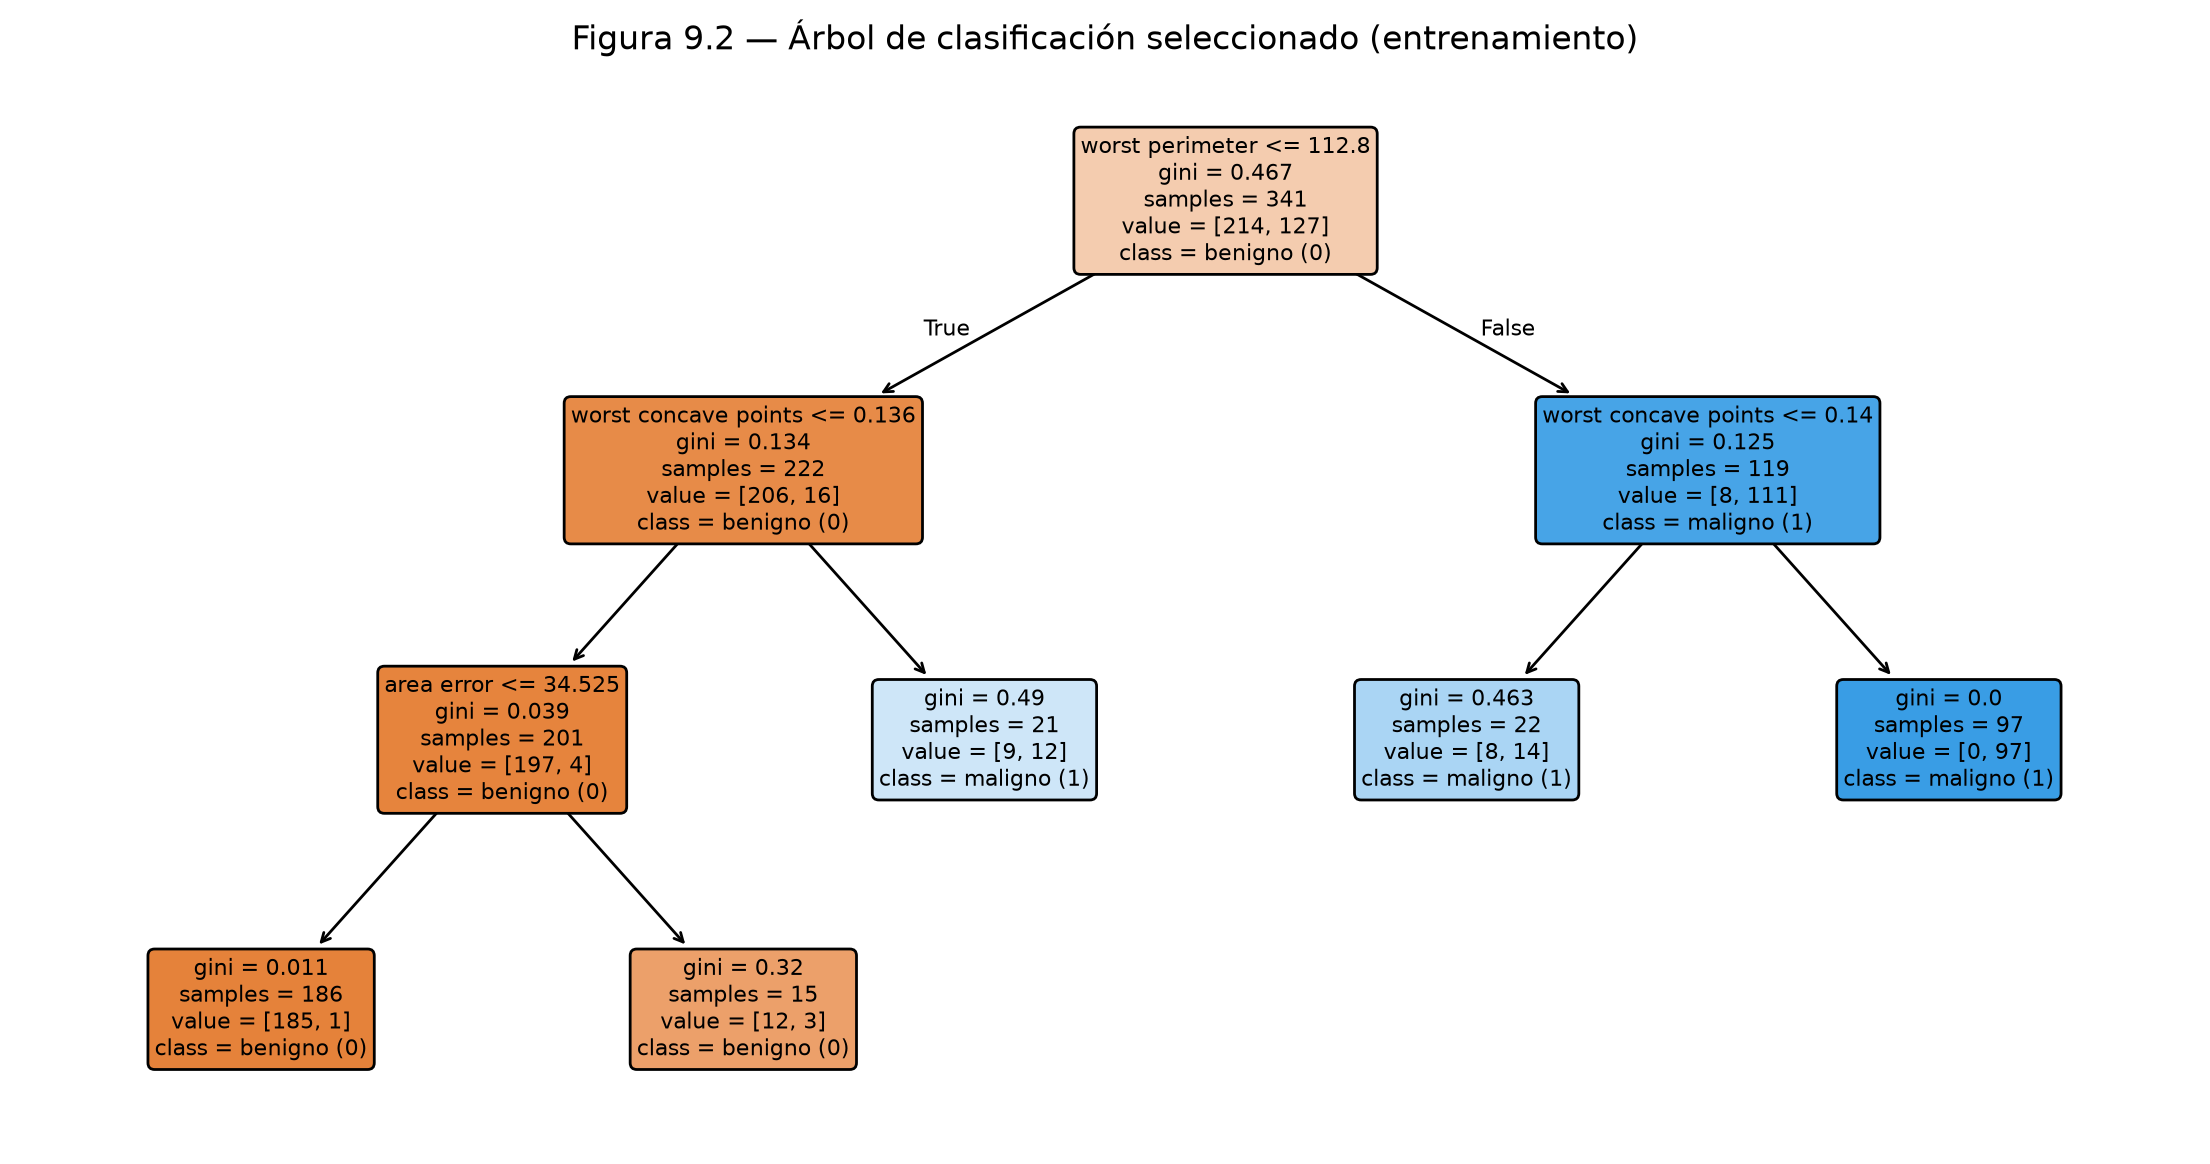
\includegraphics[width=\textwidth]{figuras/ex9_arbol.png}
    \caption{Árbol de clasificación seleccionado, ajustado con entrenamiento (conteos por clase en cada nodo).}
    \label{fig:ex9-arbol}
\end{figure}

\item \textbf{Importancias, coeficientes y sobreajuste.}
La \emph{importancia} de una variable en un árbol es cuánta impureza de
Gini (Ejercicio~5a) se redujo en total gracias a las preguntas sobre esa
variable, normalizada para que todas sumen 1. El árbol concentra casi
toda la importancia en \texttt{worst perimeter} ($\ImpPerimetro$) y
\texttt{worst concave points} ($\ImpPuntos$), con un aporte marginal de
\texttt{area error} ($\ImpAreaError$), y solo $\ImpNoNulas$ de los 30
predictores tienen importancia distinta de cero
(Figura~\ref{fig:ex9-imp} y Tabla~\ref{tab:ex9-imp}). La regresión
logística, en cambio, reparte el peso entre muchas variables, y nos
sorprendió que \texttt{worst perimeter} ocupe apenas el puesto
$\RangoPerimetro$ por tamaño de coeficiente y \texttt{worst concave
points} el $\RangoPuntos$.

Sin embargo, las dos cosas no se pueden comparar directamente. La
importancia nunca es negativa ni tiene signo (no dice si la variable sube o
baja el riesgo), y depende de qué variable eligió primero el árbol entre
varias casi intercambiables: perímetro, radio y área miden casi lo mismo,
así que si el árbol usa una, las otras ya no aportan y quedan en cero. El
coeficiente logístico, por su parte, es un cambio en log-odds por
desviación estándar, con signo y condicional a las demás variables. Ninguno
de los dos implica efectos causales.

\begin{figure}[H]
    \centering
    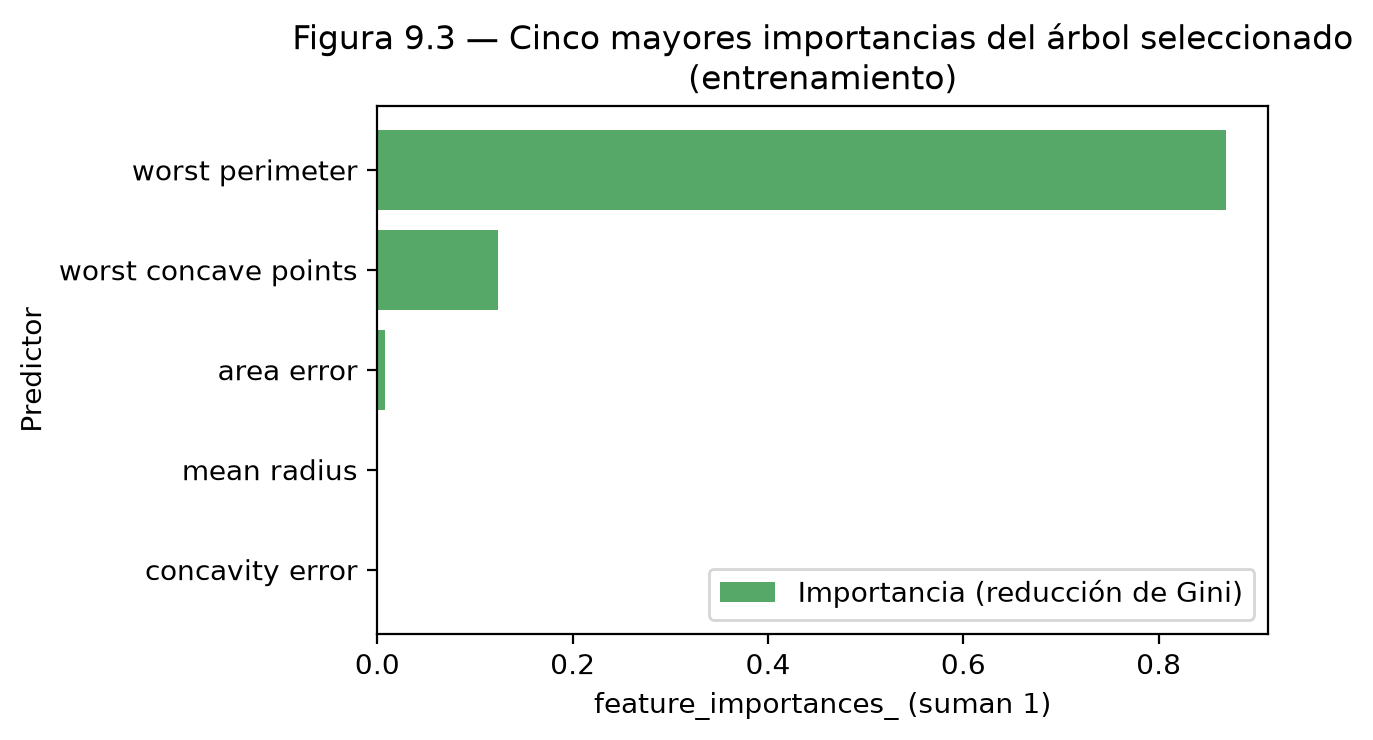
\includegraphics[width=0.66\textwidth]{figuras/ex9_importancias.png}
    \caption{Cinco mayores importancias del árbol seleccionado (entrenamiento).}
    \label{fig:ex9-imp}
\end{figure}

\begin{table}[H]
\centering
\small
% Archivo generado automáticamente por el notebook (no editar a mano).
\begin{tabular}{lrrr}
\toprule
Predictor & Importancia árbol & Coef. logística & Rango $|\beta|$ logística \\
\midrule
worst perimeter & 0.8686 & 0.6617 & 11 \\
worst concave points & 0.1234 & 0.5368 & 15 \\
area error & 0.0080 & 0.7822 & 7 \\
mean radius & 0.0000 & 0.4942 & 18 \\
concavity error & 0.0000 & $-$0.0964 & 28 \\
\bottomrule
\end{tabular}

\caption{Importancias del árbol frente a coeficientes estandarizados de la logística.}
\label{tab:ex9-imp}
\end{table}

En cuanto al sobreajuste, la Tabla~\ref{tab:ex9-arboles} muestra evidencia
clara en los árboles con \texttt{min\_samples\_leaf} $=1$, en especial el
árbol sin restricciones, que pasó de ROC-AUC $\ArbolLibreAUCTr$ y F1
$\ArbolLibreFUnoTr$ en entrenamiento a $\ArbolLibreAUCVal$ y
$\ArbolLibreFUnoVal$ en validación: perfecto con lo que ya vio, bastante
peor con lo nuevo. Los árboles con \texttt{min\_samples\_leaf} $=15$,
incluido el seleccionado (ROC-AUC de $\ArbolClfAUCTr$ en entrenamiento y
$\ArbolClfAUCVal$ en validación), fueron los que mejor trasladaron su
desempeño a validación.

\end{enumerate}

% =====================================================================
% ejercicio10.tex
% Responsabilidad única: registrar los candidatos congelados, evaluarlos una única vez en prueba
% y redactar la recomendación final.
% Las cifras provienen de generado/resultados.tex y generado/tabla_*.tex.
% =====================================================================
\subsection{Ejercicio 10: Evaluación final y recomendación sustentada}

Antes de abrir la prueba dejamos registrados los candidatos finales
(Tabla~\ref{tab:ex10-candidatos}), ambos con todos los predictores de su
caso, y conservamos los modelos tal como quedaron ajustados con
entrenamiento.

\begin{table}[H]
\centering
\resizebox{\textwidth}{!}{% Archivo generado automáticamente por el notebook (no editar a mano).
\begin{tabular}{lllll}
\toprule
Caso & Candidato final & Hiperparámetros & Umbral & Criterio de validación \\
\midrule
A (regresión) & Regresión múltiple (10 predictores) & StandardScaler + LinearRegression & — & RMSE = 51.1937 \\
B (clasificación) & Regresión logística (C = 1) & StandardScaler + LogisticRegression(C=1, lbfgs, L2) & 0.7 & L = 5 \\
\bottomrule
\end{tabular}
}
\caption{Candidatos finales congelados, decididos con validación.}
\label{tab:ex10-candidatos}
\end{table}

\begin{enumerate}

\item \textbf{Regresión en prueba.}

\begin{table}[H]
\centering
\resizebox{\textwidth}{!}{% Archivo generado automáticamente por el notebook (no editar a mano).
\begin{tabular}{lrrrrl}
\toprule
Modelo & MAE & RMSE & $R^2$ & RMSE val. & Elegido \\
\midrule
Constante (media) & 63.5314 & 72.9002 & $-$0.0031 & 75.6392 &  \\
Regresión simple (bmi) & 51.9829 & 63.8336 & 0.2309 & 58.5671 &  \\
Regresión múltiple (10 predictores) & 42.9245 & 54.1564 & 0.4464 & 51.1937 & $\checkmark$ \\
Árbol (max\_depth=4, min\_samples\_leaf=30) & 44.8448 & 58.2134 & 0.3604 & 56.7789 &  \\
\bottomrule
\end{tabular}
}
\caption{Modelos de regresión en prueba, con el RMSE de validación como referencia.}
\label{tab:ex10-reg}
\end{table}

La regresión múltiple siguió siendo la mejor en prueba (RMSE de
$\TestMultiRMSE$ y $R^2$ de $\TestMultiRdos$), seguida del árbol
($\TestArbolRegRMSE$), el modelo simple ($\TestSimpleRMSE$) y la constante
($\TestDummyRMSE$), el mismo orden que en validación
(Tabla~\ref{tab:ex10-reg}). El candidato elegido pasó de un RMSE de
validación de $\CandidatoRegRMSEVal$ a uno de prueba de
$\CandidatoRegRMSETest$, y su $R^2$ de $\RegMultiRdosVal$ a
$\TestMultiRdos$. Esa caída no nos tomó por sorpresa, porque desde el
Ejercicio~6 habíamos notado que la validación resultó una partición algo más
favorable para todos los modelos, y en cualquier caso no cambiamos de
candidato a la luz de estos resultados.

\item \textbf{Clasificación en prueba.}

\begin{table}[H]
\centering
\small
% Archivo generado automáticamente por el notebook (no editar a mano).
\begin{tabular}{llrrrr}
\toprule
Modelo & Umbral & Precisión & Recall & F1 & ROC-AUC \\
\midrule
Referencia (prior) & 0.5 & 0.0000 & 0.0000 & 0.0000 & 0.5000 \\
Regresión logística (C = 1) & 0.7 & 1.0000 & 0.9286 & 0.9630 & 0.9954 \\
Árbol (max\_depth=3, min\_samples\_leaf=15) & 0.2 & 0.8542 & 0.9762 & 0.9111 & 0.9730 \\
\bottomrule
\end{tabular}

\caption{Clasificación en prueba con los umbrales congelados: métricas.}
\label{tab:ex10-clf-met}
\end{table}

\begin{table}[H]
\centering
\small
% Archivo generado automáticamente por el notebook (no editar a mano).
\begin{tabular}{llrrrrr}
\toprule
Modelo & Umbral & TN & FP & FN & TP & Costo L \\
\midrule
Referencia (prior) & 0.5 & 72 & 0 & 42 & 0 & 210 \\
Regresión logística (C = 1) & 0.7 & 72 & 0 & 3 & 39 & 15 \\
Árbol (max\_depth=3, min\_samples\_leaf=15) & 0.2 & 65 & 7 & 1 & 41 & 12 \\
\bottomrule
\end{tabular}

\caption{Clasificación en prueba con los umbrales congelados: errores y costo $L=FP+5FN$.}
\label{tab:ex10-clf-cost}
\end{table}

La regresión logística con $t=\LogitT$ obtuvo en prueba precisión
$\TestLogitPrec$, recall $\TestLogitRecall$, F1 $\TestLogitFUno$ y ROC-AUC
$\TestLogitAUC$, con $FP=\TestLogitFP$ y $FN=\TestLogitFN$
($L=\TestLogitCosto$), mientras que el árbol con $t=\ArbolT$ obtuvo
precisión $\TestArbolClfPrec$, recall $\TestArbolClfRecall$, F1
$\TestArbolClfFUno$ y ROC-AUC $\TestArbolClfAUC$, con $FP=\TestArbolClfFP$ y
$FN=\TestArbolClfFN$ ($L=\TestArbolClfCosto$); la referencia predice todo
benigno y acumuló $L=\TestDummyCosto$. Aquí vino la parte incómoda: en
prueba el árbol tuvo un costo algo menor que el candidato elegido. La
diferencia se explica por los falsos negativos adicionales de la logística,
compensados solo en parte por sus menos falsos positivos, y coincide con la
advertencia que dejamos en el Ejercicio~8c sobre un umbral alto elegido con
pocos malignos de validación. Lo discutimos y decidimos mantener el
candidato, pues la decisión la tomamos con validación y cambiarla ahora
sería usar la prueba para seleccionar; además, con $\NClfTest$ muestras una
diferencia de pocas unidades de costo es compatible con la variabilidad
muestral, y la logística conserva un ROC-AUC claramente superior.

\paragraph{Incertidumbre de la evaluación final.}
No quisimos quedarnos solo con afirmar esa variabilidad, así que la
cuantificamos: remuestreamos con reemplazo cada conjunto de prueba
($B=\BootB$ réplicas, semilla $\Semilla$) recalculando las métricas con las
\emph{mismas predicciones congeladas}, sin reajustar nada, y comparamos los
modelos mediante diferencias \emph{pareadas} (ambos evaluados sobre la misma
réplica), que descuentan la variabilidad común (Tabla~\ref{tab:ex10-boot} y
Figura~\ref{fig:ex10-boot}).

\begin{table}[H]
\centering
\small
% Archivo generado automáticamente por el notebook (no editar a mano).
\begin{tabular}{lrrr}
\toprule
Cantidad & Puntual & IC 95 \% inf. & IC 95 \% sup. \\
\midrule
RMSE regresión múltiple & 54.1564 & 46.4859 & 61.7067 \\
RMSE árbol de regresión & 58.2134 & 49.0516 & 66.7298 \\
RMSE regresión simple & 63.8336 & 55.0919 & 72.5263 \\
$\Delta$ RMSE múltiple $-$ árbol & $-$4.0570 & $-$12.2259 & 3.5369 \\
$\Delta$ RMSE múltiple $-$ simple & $-$9.6771 & $-$17.5818 & $-$2.0302 \\
ROC-AUC logística & 0.9954 & 0.9839 & 1.0000 \\
ROC-AUC árbol & 0.9730 & 0.9410 & 0.9960 \\
Costo L logística & 15 & 0 & 35 \\
Costo L árbol & 12 & 3 & 24 \\
$\Delta$ L logística $-$ árbol & 3 & $-$16 & 27 \\
\bottomrule
\end{tabular}

\caption{Intervalos bootstrap percentiles al 95\,\% en prueba
($B=\BootB$, predicciones congeladas).}
\label{tab:ex10-boot}
\end{table}

\begin{figure}[H]
    \centering
    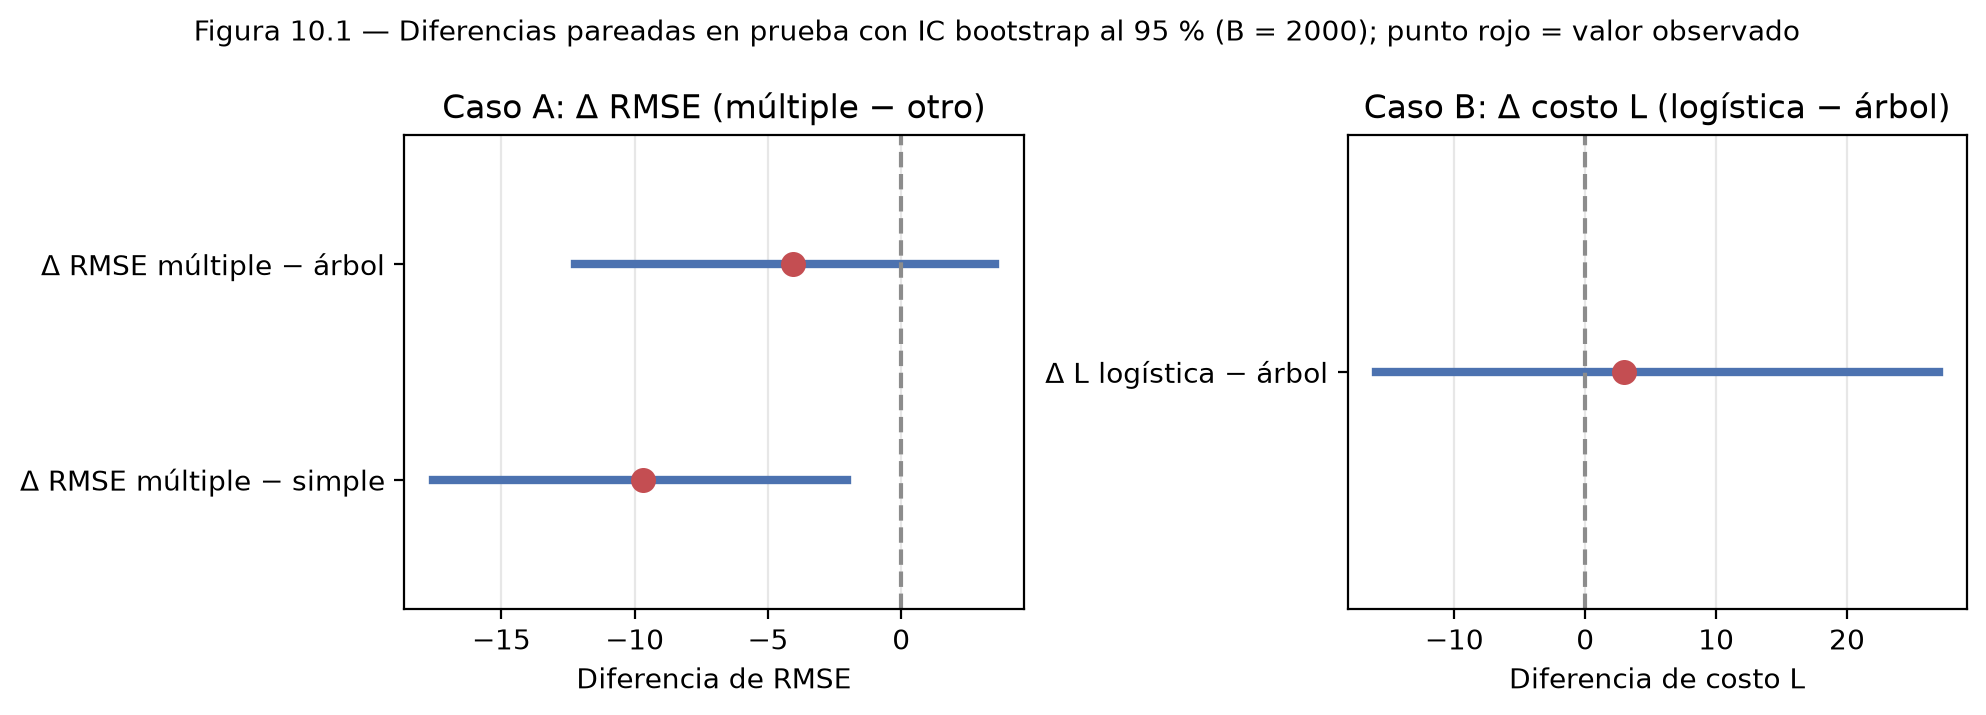
\includegraphics[width=\textwidth]{figuras/ex10_bootstrap.png}
    \caption{Diferencias pareadas en prueba con su intervalo bootstrap al
    95\,\%; si el intervalo cruza la línea punteada (cero), la prueba no
    permite distinguir a los dos modelos.}
    \label{fig:ex10-boot}
\end{figure}

En el caso A la regresión múltiple superó a la simple con un intervalo para
la diferencia de RMSE de $[\BootDifRMSEMultiSimpleInf,\ \BootDifRMSEMultiSimpleSup]$,
que excluye el cero, de forma que esa mejora es robusta, mientras que frente
al árbol el intervalo $[\BootDifRMSEMultiArbolInf,\ \BootDifRMSEMultiArbolSup]$
sí incluye el cero, por lo cual la prueba por sí sola no nos permite afirmar
que la múltiple sea mejor que el árbol (la elección se sostiene en la
validación y en su menor complejidad). En el caso B la diferencia pareada de
costo (logística menos árbol) fue de $\BootDifLLogitArbolInf$ a
$\BootDifLLogitArbolSup$, con la logística más costosa en una fracción
$\BootPropLogitPeor$ de las réplicas, es decir, la ventaja del árbol en
prueba es compatible con el azar del muestreo, mientras que la superioridad
de la logística en ordenamiento es más clara (ROC-AUC con intervalo
$[\BootAUCLogitInf,\ \BootAUCLogitSup]$ frente a
$[\BootAUCArbolInf,\ \BootAUCArbolSup]$ del árbol). Los intervalos de $L$
salieron tan anchos porque $L$ depende de unos pocos falsos negativos que
valen 5 cada uno.

\item \textbf{Matrices de confusión y costo.}

\begin{figure}[H]
    \centering
    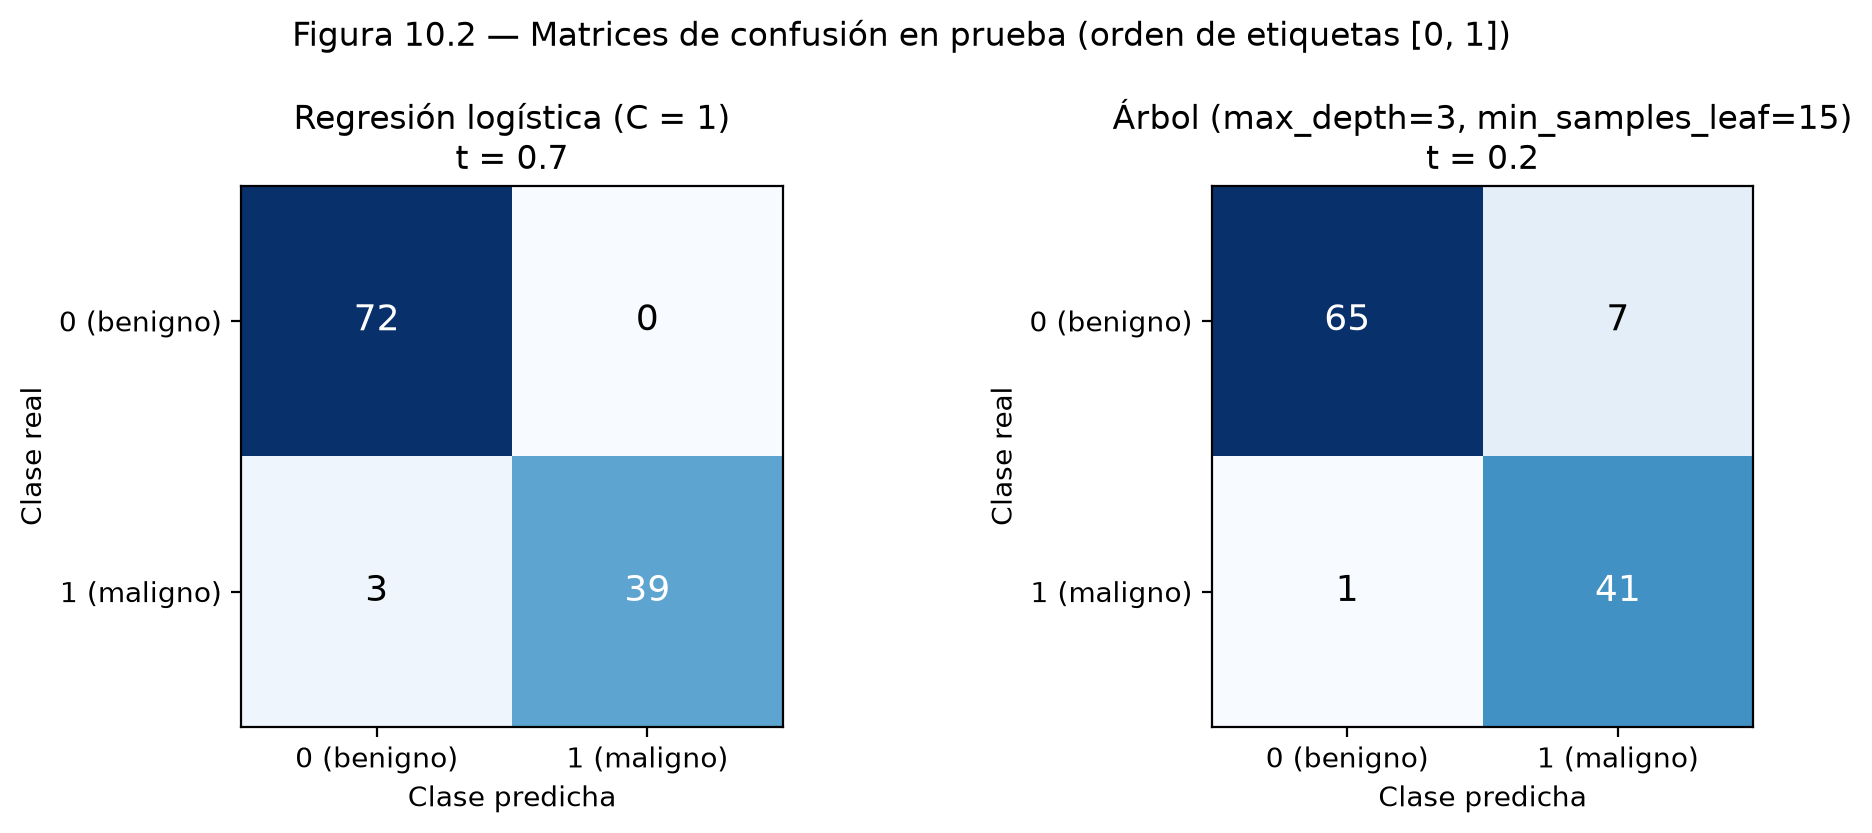
\includegraphics[width=\textwidth]{figuras/ex10_matrices_confusion.png}
    \caption{Matrices de confusión en prueba, filas reales y columnas predichas en orden $[0,1]$.}
    \label{fig:ex10-cm}
\end{figure}

En este conjunto, un \textbf{falso positivo} es una muestra de tejido
benigno clasificada como maligna, lo que en un uso hipotético implicaría
exámenes adicionales innecesarios y angustia para la paciente, mientras que
un \textbf{falso negativo} es una muestra maligna clasificada como benigna,
lo que retrasaría un diagnóstico y un tratamiento, consecuencia mucho más
grave y razón por la cual el costo didáctico la pondera cinco veces. Para el
candidato elegido, la matriz de la Figura~\ref{fig:ex10-cm} quedó con
$TN=\TestLogitTN$, $FP=\TestLogitFP$, $FN=\TestLogitFN$ y $TP=\TestLogitTP$,
de modo que
\[
    L = FP + 5\,FN = \TestLogitFP + 5\cdot\TestLogitFN = \TestLogitCosto,
\]
valor que coincide con la Tabla~\ref{tab:ex10-clf-cost}.

\item \textbf{Recomendación.}
% Versión en primera persona del texto de la celda 10d del notebook (allí
% se verifica el rango exigido de 250 a 350 palabras).
Para el caso A (progresión de la diabetes) recomendamos la regresión lineal
múltiple con los diez predictores estandarizados, pues fue el candidato con
menor RMSE de validación ($\CandidatoRegRMSEVal$) y conservó el primer lugar
en prueba (RMSE de $\TestMultiRMSE$ y $R^2$ de $\TestMultiRdos$), por delante
del árbol y de la regresión simple con \texttt{bmi}. Además es interpretable,
ya que cada coeficiente se lee como el cambio esperado ante una desviación
estándar del predictor, con el detalle de que la fuerte correlación entre
\texttt{s1} y \texttt{s2} impide leer esos coeficientes como importancias
independientes o como efectos causales, y un $R^2$ cercano a
$\TestMultiRdos$ indica que más de la mitad de la variabilidad queda sin
explicar.

Para el caso B (clasificación de tejido) recomendamos la regresión logística
con $C=\LogitC$ y umbral $\LogitT$, que elegimos por menor costo en
validación ($L=\LogitCostoSel$) y que en prueba obtuvo ROC-AUC de
$\TestLogitAUC$, precisión de $\TestLogitPrec$ y recall de
$\TestLogitRecall$, aunque con $L=\TestLogitCosto$ frente a
$L=\TestArbolClfCosto$ del árbol, diferencia que con $\NClfTest$ muestras de
prueba no justifica cambiar de candidato después de ver los resultados. El
árbol, más simple de explicar con dos o tres reglas, sacrifica capacidad de
ordenamiento y depende de pocas variables.

Si un candidato rinde peor en prueba que en validación, como nos pasó en
ambos casos, lo reportamos tal cual como estimación honesta y, en lugar de
reajustar con prueba, revisamos el análisis sobre el conjunto de desarrollo
y, de ser necesario, reservamos un nuevo conjunto de prueba.

Nos quedan dos limitaciones. Primero, los tamaños son pequeños ($\NRegVal$ y
$\NClfVal$ observaciones de validación), por lo que umbrales y empates
dependen de unos pocos casos. Segundo, los datos son observacionales y de
una sola fuente, sin evaluación externa ni costos clínicos reales detrás de
$L=FP+5FN$. Como mejora futura proponemos elegir hiperparámetros y umbral con
validación cruzada estratificada dentro del conjunto de desarrollo, menos
sensible a una sola partición, y luego evaluar en una cohorte externa.

\end{enumerate}


% ---------------------------------------------------------------------
% Apéndice — Entorno de ejecución
% ---------------------------------------------------------------------
\newpage
\appendix
% =====================================================================
% apendice.tex
% Responsabilidad única: registrar el entorno de ejecución (versiones y
% semilla), como pide el protocolo del taller. Las versiones son macros
% que escribe el notebook al ejecutarse.
% =====================================================================
\section{Entorno de ejecución}
\label{sec:entorno}

Los resultados de la Parte II los obtuvimos con el entorno de la
Tabla~\ref{tab:entorno}, que el propio notebook registra al ejecutarse.
Dado que los modelos que usamos (regresiones por mínimos cuadrados, logística
con \texttt{lbfgs} y árboles con \texttt{random\_state} fijo) son
deterministas una vez fijada la partición, una reejecución con estas
versiones reproduce exactamente las mismas cifras, mientras que con otras
versiones de scikit-learn podrían aparecer diferencias en los últimos
decimales.

\begin{table}[H]
\centering
\small
\begin{tabular}{ll}
\toprule
Componente & Versión / valor \\
\midrule
Python        & \VerPython \\
NumPy         & \VerNumpy \\
pandas        & \VerPandas \\
Matplotlib    & \VerMatplotlib \\
scikit-learn  & \VerSklearn \\
Semilla (\texttt{random\_state} y bootstrap) & \Semilla \\
\bottomrule
\end{tabular}
\caption{Entorno de ejecución de la Parte II.}
\label{tab:entorno}
\end{table}


\end{document}
